\documentclass[hidelinks, 12pt]{report}
\usepackage{fontspec}
\usepackage{xunicode}
\usepackage[french]{babel}

\usepackage{csquotes}
\usepackage[style=verbose-ibid,backend=bibtex]{biblatex}

\usepackage{titlesec}
\titleformat{\chapter}{}{}{0em}{\bf\LARGE}
\usepackage{caption}
\usepackage{hyperref}
\usepackage{enumitem}
\usepackage{setspace}
\usepackage{lscape}
\usepackage{graphicx}
\usepackage{float}

\usepackage{soul}
\usepackage{color}
\usepackage[dvipsnames]{xcolor}
\usepackage{listings}

\newcommand{\code}[1]{\colorbox{LightGray}{\texttt{#1}}}

\definecolor{LightGray}{rgb}{0.97,0.97,0.97}
\definecolor{red}{RGB}{255,0,0}
\definecolor{brown}{RGB}{139,69,19}
\definecolor{green}{RGB}{0,128,0}
\definecolor{blue}{RGB}{0,0,255}

\lstdefinelanguage{SPARQL}{
	basicstyle=\small\ttfamily,
	backgroundcolor=\color{LightGray},
	%	
	tabsize=1,
	showstringspaces=false,
	columns=fullflexible,
	breaklines=true,
	breakatwhitespace=true,
	%
	aboveskip=1em,
	belowskip=1em,
	xleftmargin=.5em,
	xrightmargin=.5em,
	framexleftmargin=.5em,
	framextopmargin=.5em,
	framexbottommargin=.5em,
	framexrightmargin=.5em,
	%
	morekeywords=[1]{paysLabel,population,date,cio,pays,populationStatement,noc,geopoint,RegionLabel,Region},
	keywordstyle=[1]\color{green},
	%
	morekeywords=[2]{wd,Q6256,wdt,P31,p,P1082,ps,pq,P585,wikibase,P984,label,bd,serviceParam,language,P625,Q36784,Q48091},
	keywordstyle=[2]\color{MidnightBlue},
	%
	morekeywords=[3]{SELECT,ORDER,BY,WHERE,FILTER,YEAR,NOW,SERVICE,DISTINCT},
	keywordstyle=[3]\color{red},
	%
	morestring=[b][\color{brown}]",
	otherkeywords={?},
}

\lstdefinelanguage{python}{
	basicstyle=\small\ttfamily,
	backgroundcolor=\color{LightGray},
	%	
	tabsize=1,
	showstringspaces=false,
	columns=fullflexible,
	breaklines=true,
	breakatwhitespace=true,
	%
	aboveskip=1em,
	belowskip=1em,
	xleftmargin=.5em,
	xrightmargin=.5em,
	framexleftmargin=.5em,
	framextopmargin=.5em,
	framexbottommargin=.5em,
	framexrightmargin=.5em,
	%
	morekeywords=[1]{import,as,for,in,True},
	keywordstyle=[1]\color{Fuchsia},
	%
	morekeywords=[2]{FMI\_prepared2,FMI\_prepared2\_df,colonnes\_a\_traiter,colonne,condition,keep,subset,FMI\_Python},
	keywordstyle=[2]\color{MidnightBlue},
	%
	morekeywords=[3]{dataiku,pandas,pd},
	keywordstyle=[3]\color{green},
	%
	morestring=[b][\color{brown}]",
	morestring=[b][\color{brown}]',
}


\lstdefinelanguage{tableau}{
	basicstyle=\small\ttfamily,
	backgroundcolor=\color{LightGray},
	%	
	tabsize=1,
	showstringspaces=false,
	columns=fullflexible,
	breaklines=true,
	breakatwhitespace=true,
	%
	aboveskip=1em,
	belowskip=1em,
	xleftmargin=.5em,
	xrightmargin=.5em,
	framexleftmargin=.5em,
	framextopmargin=.5em,
	framexbottommargin=.5em,
	framexrightmargin=.5em,
	%
	morekeywords=[3]{YEAR},
	keywordstyle=[3]\color{DarkOrchid},
	%
	morekeywords=[2]{Medals,1996,2000,2004,2008,2012,2016,-},
	keywordstyle=[2]\color{Bittersweet},
	%
	morekeywords=[1]{[,]},
	keywordstyle=[1]\color{OliveGreen},
	%
	otherkeywords={1996,2000,2004,2008,2012,2016,-,[,]},
}

\bibliography{Journal-de-bord-bibliographie}

\title{Projet Jeux Olympiques - Journal de bord}
\date{Janvier 2024}
\author{T. Burnel, N. Grim, M. Griveau, M. Mechentel}

\begin{document}

\setstretch{1.5}
\maketitle





%





\tableofcontents

\chapter{Introduction}

Nous sommes une équipe de datajournalistes chargée, à l'approche des Jeux Olympiques de Paris, d'étudier l'existence ou non de liens entre le succès d'un pays aux Jeux et sa richesse. Notre hypothèse de départ est la suivante : les pays développés gagnent significativement plus de médailles en raison de leur niveau d'investissement dans le domaine sportif.

À l'aune de l'examen et du traitement des données que nous avons à notre disposition, nous avons pour ambition d'apprécier l'influence de la politique d'investissement dans les infrastructures sportives des pays sur leurs résultats aux épreuves des Jeux Olympiques.

Notre travail sera divisé en deux temps. Nous mettrons en relief le nombre de médailles remportées par les pays lors de six éditions des Jeux (1996, 2000, 2004, 2008, 2012, 2016) par rapport à leur population, à leur Produit Intérieur Brut et au pourcentage de ce dernier investi dans le domaine sportif. Un second temps sera consacré à l'examen de la réussite de la France et du Royaume-Uni aux épreuves de natation sur la base du nombre d'infrastructures relatives pour 100.000 habitants sur leur territoire. Cette petite nuance au sein de notre jeu nous permettra d'éprouver notre hypothèse volontairement générale, mais pour autant pertinente.

Le choix de ces pays repose sur divers points de convergence : leur nombre d'habitants, leur économie et leur qualité de pays organisateur des Jeux. L'échelle localisée de l'étude trouve ici sa pertinence.

Travailler sur une période de vingt ans nous semble suffisant pour cerner ou non le début d'une tendance économique vis-à-vis de la réussite des pays aux Jeux Olympiques. Le temps et les ressources dont nous disposons tendent à confirmer le choix de cette période -- suffisamment éloquente en données pour nous permettre de travailler avec un matériau d'une qualité et d'une quantité honorables sans qu'il ne faille faire entorse à nos capacités financières -- strictement égales à zéro -- et humaines -- strictement égales à quatre.

Nous sommes \textit{ipso facto} conscients de la prudence dont nous devrons faire preuve, le moment des conclusions venu. Il s'agit bien davantage d'un travail préliminaire que la rigueur journalistique force à éprouver et à approfondir que d'une parole d'évangile dispensable de toute remise en question.

Le résultat du traitement des données, réalisé sur le logiciel Dataiku, constituera une base à la conception de datavisualisations sur le logiciel Tableau Public et d'une application web exploitables pour l'écriture d'articles journalistiques sur le sujet des Jeux Olympiques. Les données mises à disposition, exception faite du nom des régions de France, sont en langue anglaise dans l'idée d'une exploitation par la presse internationale.





%





\chapter{Jeux de données}

\section{Jeux du premier flux}

Notre premier flux concerne les médailles remportées par les pays lors des six éditions des Jeux Olympiques que nous avons retenues. En amont du traitement, nos jeux étaient au nombre de deux. Le premier présente le nombre de médailles remportées par sportif aux Jeux sur une période de 120 ans\autocite{kaggle}. Le deuxième, le Produit Intérieur Brut des pays et son pourcentage investi dans le domaine sportif\autocite{fmi}.

Nous avons enrichi ces jeux grâce au résultat d'une requête SPARQL, saisie sur le service de Wikidata. Le jeu ainsi produit présente le nombre d'habitants de l'ensemble des pays répertoriés dans la base de données de Wikidata, sur une période de trente ans (1993 - 2023)\autocite{wikiquerypop}.

Trois autres jeux ont dû faire leur entrée au cours du traitement pour pallier de nombreux manquements. Nous avons constaté qu'en dépit d'indiquer le pourcentage du Produit Intérieur Brut investi dans le domaine sportif, le jeu du Fonds Monétaire International ne contenait pas le PIB des pays. Nous avons introduit un jeu de la Banque mondiale\autocite{worldbank} dans le flux -- lequel contient le montant du PIB avec une profondeur chronologique suffisante.

Les deux autres jeux concernent un problème de coordonnées. Lorsque Dataiku identifie des données de type \textit{country}, nous pensions pouvoir en récupérer les coordonnées -- notamment afin de les exploiter pour les datavisualisations. L'extension \textit{reverse geocoding plugin} aurait pu nous le permettre, sans succès. Nos suppositions portent sur notre version gratuite de Dataiku et de son nombre réduit de fonctionnalités.

Ne disposant d'aucun budget pour bénéficier d'une version payante, nous avons recherché un jeu contenant les coordonnées des pays et l'avons trouvé sur la plateforme GitHub\autocite{github}. Nonobstant, les longitudes et latitudes des pays ainsi récupérées se sont avérées être fautives le moment des datavisualisations venu. C'est pourquoi nous avons mis au point une deuxième requête SPARQL, capable de renvoyer les bonnes coordonnées de tous les pays présents dans la base de Wikidata\autocite{wikiquerycoor}. Le jeu ainsi récupéré correspond au dernier renfort dont nous avons eu besoin pour réaliser les datavisualisations.





%





\subsection{Jeu de Kaggle}\label{kaggle}

Le jeu est composé de 15 colonnes et 271.117 lignes. 7 colonnes fournissent des informations sur les athlètes (\textit{ID}, \textit{Name}, \textit{Sex}, \textit{Age}, \textit{Height}, \textit{Weight}, \textit{Medal}) ; 2 colonnes sur leurs pays (\textit{Team}, \textit{NOC}) et 6 sur les éditions des Jeux Olympiques (\textit{Games} ; \textit{Year} ; \textit{Season} ; \textit{City} ; \textit{Sport} ; \textit{Event}).

Les données sont exprimées en langue anglaise. La casse des chaînes de caractères suit le schéma d'une majuscule à chaque nouveau mot -- exception faite des unités de mesure dans la colonne \textit{Event} (comprendre \textit{Épreuve}) : le terme \enquote{metres} est toujours noté en bas-de-casse. 2 colonnes, \textit{Games} et \textit{Year} contiennent des données de date, exprimées en année. La colonne \textit{Games} a pour particularité d'agréger une donnée de date et une donnée textuelle. Les Jeux Olympiques d'été de 1992 sont ainsi notés \enquote{1992 Summer}.

Le jeu ne présente pas de défauts majeurs sur les colonnes que nous comptons conserver lors du traitement. Un problème plus préoccupant concerne la dénomination des pays, parfois obsolète (\enquote{Soviet Union}, \enquote{West Germany}) ou impropres (\enquote{Japan-1}, \enquote{Switzerland-2}). Nous effectuerons les jointures sur le code NOC des pays (un code unique attribué par le Comité National Olympique) pour plus de fiabilité.





%





\subsection{Jeu du FMI}

Le jeu est composé de 42 colonnes pour 7.715 lignes. La colonne \textit{Country Name} permet d'identifier les pays. Celle nommée \textit{COFOG Function Name} correspond au secteur des investissements et a pour unique valeur \textit{Expenditure on recreational \& sporting services} -- car nous avions sollicité l'API du FMI en demandant l'unique fonction COFOG numérote 8.1, laquelle correspond aux investissements dans le domaine sportif. La colonne \textit{Unit Name} précise l'échelle de calcul des investissements (soit en pourcentage du PIB, \textit{Percent of GDP}, soit en monnaie courante \textit{Domestic currency}). Le montant des investissements est renseigné sur 30 colonnes, de 1993 à 2022.

Les 9 autres colonnes correspondent à des codes et des dénominations propres au FMI (\textit{Country Code}, \textit{COFOG Function Code}, \textit{Sector Name}, \textit{Sector Code}, \textit{Unit Code}, \textit{Attribute}, \textit{Indicator Code}, \textit{Global DSD Time Series Code}, \textit{col\_41}). Le potentiel de croisement avec d'autres jeux étant par la force des choses très limité, nous n'utiliserons pas ces données.

L'ensemble du jeu est rédigé en langue anglaise. Noms de pays, sigles, codes, acronymes et unités de mesure (notées \enquote{Cash}, \enquote{Non Cash}, \enquote{Gross}, \enquote{Net}) à part, la casse des données textuelles implique la présence d'une seule majuscule en début de chaîne. Nous notons l'utilisation de caractères spéciaux, à l'instar de l'esperluette ou de la barre oblique.

Exception faite des \textit{Country Code} et du code correspondant à la valeur \enquote{Domestic currency}, l'intégralité des codes sont un mélange de caractères numériques et textuels en haut-de-casse (\enquote{S13112} pour la colonne \textit{Sector Code} ou \enquote{XDC\_R\_B1GQ} dans la colonne \textit{Unit Code}).

Les noms de pays souffrent d'un problème d'harmonisation et d'actualité (\enquote{Russian Federation}, \enquote{China, P.R.: Mainland}, etc.).

Ce jeu est de loin le moins bien structuré et le plus fautif de notre \textit{set} basal. Bien que nous ne comptions pas les conserver au cours du traitement, les trois dernières colonnes (\textit{Indicator Code}, \textit{Global DSD Time Series Code}, \textit{col\_41}) sont d'une opacité confondante et témoignent du problème majeur du jeu : beaucoup de données sont inexistantes, nulles ou incompréhensibles (\enquote{GERS\_G14\_GDP\_PT} pour la colonne \textit{Indicator Code}, \enquote{A|GB|S1311|W0|S1|G2M|\_Z|\_Z|GF0801|
	XDC|\_T|\_X} pour la colonne \textit{Global DSD Time Series Code}).

Également, au sein des colonnes qui correspondent au montant des investissements par année se côtoient des lignes vides et des sigles (\enquote{NA}, \enquote{NP}, \enquote{AC}), sans justification ni harmonisation aucune. En somme, ce jeu représente un véritable enjeu de nettoyage et de croisement des données.





%





\subsection{Jeu de Wikidata (population)}

En préambule de l'analyse du jeu de Wikidata, revenons un instant sur l'élaboration de la requête nous ayant permis de l'obtenir. Celle-ci renvoie le nombre d'habitants de l'ensemble des pays présents dans la base de données de Wikidata sur une période de trente ans (1993 - 2023) :

\label{query1}\begin{lstlisting}[language=SPARQL]
SELECT ?paysLabel ?population ?date ?cio
WHERE 
{
	?pays wdt:P31 wd:Q6256.
	?pays wdt:P984 ?cio.
	?pays p:P1082 ?populationStatement.
	?populationStatement ps:P1082 ?population. 
	?populationStatement pq:P585 ?date.
	FILTER(YEAR(?date) >= (YEAR(NOW()) - 30)).
	SERVICE wikibase:label { bd:serviceParam wikibase:language "[AUTO_LANGUAGE],fr". }
}
ORDER BY ?paysLabel ?date
\end{lstlisting}

Être en mesure de requêter l'intégralité des pays a été la première étape de la construction de notre requête. Le premier triplet permet de spécifier la nature -- notée \code{wdt:P31} -- de notre variable inconnue \code{?pays} en la faisant correspondre à l'objet \code{country} -- noté \code{wd:Q6256} :

\begin{lstlisting}[language=SPARQL]
	?pays wdt:P31 wd:Q6256.
\end{lstlisting}

Le deuxième triplet constitue un ajout tardif, destiné à faciliter les jointures avec les autres jeux de données. Comme nous travaillons sur les Jeux Olympiques, les pays peuvent être non seulement identifiés par les codes basés sur la norme ISO 3166 mais aussi par les codes du CIO (Comité International Olympique). Nous avons donc récupéré cette donnée grâce à la propriété Wikidata correspondante -- notée \code{wdt:P984} :

\begin{lstlisting}[language=SPARQL]
	?pays wdt:P984 ?cio.
\end{lstlisting}

La deuxième partie de notre requête renvoie le nombre d'habitants par pays en prenant en compte une dimension chronologique. La complexité de cette demande requiert un parcours de graphique en quatre temps.

Pour ce faire, nous avons consulté la liste de préfixes\autocite{wikiprefixes} de Wikidata afin de créer une nouvelle variable : \code{?populationStatement}. Le troisième triplet a recours à la classe \code{population} -- notée \code{p:P1082} -- et signifie que la variable \code{?populationStatement} a pour valeur la population des pays :

\begin{lstlisting}[language=SPARQL]
	?pays p:P1082 ?populationStatement.
\end{lstlisting}

L'obtention du nombre d'habitants a nécessité l'utilisation du préfixe \code{ps}, lequel permet de récupérer la valeur de la propriété relative à la population :

\begin{lstlisting}[language=SPARQL]
	?populationStatement ps:P1082 ?population.
\end{lstlisting}

Enfin, nous avons rédigé le dernier triplet sur la base du préfixe \code{pq} pour attribuer la valeur chronologique à la variable \code{?date}. Un filtre y a été appliqué pour exprimer les limites extrêmes de notre période, soit \code{NOW} pour 2023 et \code{-30} pour 1993 :

\begin{lstlisting}[language=SPARQL]
	?populationStatement pq:P585 ?date.
	FILTER(YEAR(?date) >= (YEAR(NOW()) - 30)).
\end{lstlisting}

La première et la dernière ligne permettent de cadrer l'affichage des résultats. Lorsque la requête s'exécute, Wikidata renvoie le nom de chaque pays (\code{?paysLabel}) par ordre alphabétique, le nombre d'habitants (\code{?population}) et l'année correspondante (\code{?date}) par ordre croissant :

\begin{lstlisting}[language=SPARQL]
	SELECT ?paysLabel ?population ?date
	ORDER BY ?paysLabel ?date
\end{lstlisting}

Nous nous sommes heurtés à plusieurs obstacles avant de rendre la requête fonctionnelle. Il nous a fallu un certain temps avant de comprendre la nécessité d'un parcours de graphique en quatre temps et du recours à une variable telle que \code{?paysStatement}. À cet égard, la documentation sur l'utilisation des propriétés \code{population}\autocite{wikipop} et \code{date}\autocite{wikidate} a été d'un grand secours.

Nous avons également pris en exemple la requête \emph{Population in Europe after 1960}\autocite{wiki1960}. La consulter a été l'occasion d'une meilleure compréhension des propriétés Wikidata ainsi qu'une porte ouverte à la lecture de la documentation et à l'appréhension des requêtes en deux temps (collecte des propriétés d'une classe puis requêtage en fonction de notre besoin).

La rédaction de cette première requête a été d'une grande aide pour les autres recours à Wikidata qui ont émaillé notre chaîne de traitement.
\newline

Le jeu ainsi généré est composé de 13 colonnes et 3.737 lignes. Les lignes de la colonne, \textit{paysLabel.xml:lang} sont composées d'une même et unique donnée : \enquote{fr}. Il s'agit de langue dans laquelle les noms des pays sont renvoyés. 

\label{query1tab}Sur les 12 colonnes restantes, 6 fonctionnent selon une logique de duo et 6 autres selon une logique de trio. Pour chaque donnée, le jeu indique sont \textit{type}, sa \textit{value} et, pour les trio, son \textit{datatype}. Ainsi, la donnée \enquote{cio} fait l'objet de 2 colonnes : \textit{cio.type}, \textit{cio.value} (\textit{idem} pour les données \enquote{isoCode} et \enquote{paysLabel}) et la donnée \enquote{date} fait l'objet de 3 colonnes : \textit{date.datatype}, \textit{date.type}, \textit{date.value} (\textit{idem} pour la donnée \enquote{population}). 

\label{nongrata}Bien que notre requête ne précise vouloir recueillir ni le \textit{type} ni le \textit{datatype} des données, ces colonnes sont malgré tout présentes dans le jeu de sortie. Les données textuelles sont exprimées en anglais (mis à part les noms de pays) et sont en bas-de-casse -- exception faite des sigles et des noms de pays. Les dates sont exprimées selon le schéma YYYY-MM-DDThh\!\!:mm\!\!:ssZ. L'intégralité des \textit{types} correspondent à \enquote{literal}. Les colonnes \textit{datatype} ont pour valeur des liens renvoyant à des schémas XML du W3C.

Le jeu est d'une propreté exemplaire, les données sont harmonisées et correctement typées, ce qui nous sera d'une grande aide lors des jointures. Cependant, la correcte forme des données est minée par de sérieux manques, notamment pour l'année 2016.





%





\subsection{Jeu de la Banque mondiale}

Le jeu se compose de 68 colonnes pour 533 lignes. Chaque ligne pleine est en réalité séparée de la suivante par une ligne vide. De surcroît, la dernière colonne est intégralement vide et ne porte que le sommaire nom de \textit{col\_67}. Sur l'ensemble du jeu, 63 colonnes correspondent aux années pour lesquelles le PIB des pays est renseigné (1960 - 2022). 2 autres colonnes donnent des informations sur les pays : leur nom, leur code (\textit{Country Name}, \textit{Country Code}) et les 2 restantes, sur la donnée économique -- en l'occurrence le PIB (\textit{Indicator Name}, \textit{Indicator Code}), en dollars courant. 

Les données textuelles sont en langue anglaise. Les noms des pays portent une majuscule initiale. Les codes sont exclusivement en haut-de-casse. Les données numériques sont exprimées en décimaux.

Notons que certaines entrées de la colonne \textit{Country Name} témoignent d'une certaine originalité dans la mesure où ils ne sont pas références à des pays nommément explicites (\enquote{Heavily indebted poor countries (HIPC)}, \enquote{IBRD only}, \enquote{Low \& middle income}, etc.). Ces excentricités soulignent l'importance des codes des pays pour effectuer les jointures et faire l'économie des entrées impropres. Enfin, les premières décennies souffrent d'un cruel manque de données mais plus nous avançons dans le temps, plus le jeu est complet sur l'ensemble des pays.





%





\subsection{Jeu de GitHub}

Le jeu se compose de 6 colonnes et 263 lignes. 2 de ces colonnes correspondent à la latitude et longitude (\textit{Latitude (average)}, \textit{Longitude (average)}) des pays dont le nom nous est donné dans la colonne \textit{Country}. Les trois autres colonnes (\textit{Alpha-2 code}, \textit{Alpha-3 code}, \textit{Numeric code}) correspondent à des codes de pays prévus par la norme ISO 3166-1.

Les données textuelles sont exprimées en langue anglaise. Nonobstant, nous comptons nous appuyer sur les codes des pays pour réaliser les jonctions. Le jeu ne présente aucune donnée manquante.





%





\subsection{Jeu de Wikidata (coordonnées)}

Revenons derechef sur le détail de notre requête SPARQL, rédigée pour nous permettre de récupérer les coordonnée des pays recensés dans la base de données de Wikidata :

\begin{lstlisting}[language=SPARQL]
SELECT DISTINCT ?paysLabel ?geopoint ?noc
WHERE 
{
	?pays wdt:P31 wd:Q6256.
	?pays wdt:P984 ?noc.
	?pays wdt:P625 ?geopoint
	SERVICE wikibase:label { bd:serviceParam wikibase:language "[AUTO_LANGUAGE],en". }
}
\end{lstlisting}

Nous indiquons vouloir récupérer les données selon les colonnes suivantes : le nom du pays (noté \code{?paysLabel}), leurs coordonnées (notées \code{?geopoint}) et leur code CIO (noté \code{?noc}) :

\begin{lstlisting}[language=SPARQL]
	SELECT DISTINCT ?paysLabel ?geopoint ?noc
\end{lstlisting}

Le premier triplet est \textit{stricto sensu} le même que celui de notre première requête Wikidata sur les populations (\textit{cf}. \textit{supra} p. \pageref{query1}).

Il permet de signifier que notre variable inconnue \code{?pays} est de nature (notée \code{wdt:P31}) \enquote{pays} (noté \code{wd:Q6256}) :

\begin{lstlisting}[language=SPARQL]
	?pays wdt:P31 wd:Q6256.
\end{lstlisting}

Le deuxième triplet est également tout à fait similaire à son homonyme de la requête sur les populations (\textit{cf}. \textit{supra} p. \pageref{query1}). Il assigne à la variable \code{?noc} les codes des pays prévus par le Comité Olympique International grâce à la propriété relative notée \code{wdt:P984} :

\begin{lstlisting}[language=SPARQL]
	?pays wdt:P984 ?noc.
\end{lstlisting}

Enfin, le dernier triplet récupère les coordonnées géographiques des pays grâce à la propriété correspondante, notée \code{wdt:P625} :

\begin{lstlisting}[language=SPARQL]
	?pays wdt:P625 ?geopoint
\end{lstlisting}

Il en ressort un jeu composé de 8 colonnes et 185 lignes. Il présente la même logique de duo et de trio que notre autre jeu Wikidata (\textit{cf}. \textit{supra} p. \pageref{query1tab}) : les données \enquote{noc} et \enquote{paysLabel} font l'objet de 2 colonnes et les coordonnées, \enquote{geopoint}, font l'objet de 3 colonnes. La longitude et la latitude sont regroupées au sein de la même colonne, \textit{geopoint.value} et sont présentées comme suit : \enquote{Point(<longitude> <latitude>)}. L'Islande a ainsi pour coordonnées \enquote{Point(-19.0 65.0)}.

Cette requête ayant été saisie dans l'urgence de devoir déboguer la réalisation des datavisualisations et la rédaction du présent journal de bord à moins d'une semaine de la date butoir, les noms de pays sont exprimés en langue anglaise et les résultats n'ont pas été ordonnés par ordre alphabétique à l'instar de la requête sur la population. Nonobstant, la forme des données qui nous préoccupent -- en l'occurrence, les codes NOC et les coordonnées -- ne dépend pas de la langue pourvu que l'alphabet soit le même.





%





\section{Jeux du second flux}

Notre deuxième flux repose sur une comparaison entre la France et le Royaume-Uni à propos de la natation. En amont du traitement, nos jeux étaient au nombre de cinq : trois pour le Royaume-Uni, deux pour la France.

Sur le Royaume-Uni, un premier jeu résulte d'une requête SPARQL, laquelle génère un jeu listant le nom des régions du pays, leur nombre d'habitants et leurs coordonnées\autocite{wikiqueryeng}. Les deux autres jeux proviennent du même site\autocite{ru}, l'un situe les infrastructures sportives par rapport à leur région, l'autre les décrit d'un point de vue davantage technique.

Sur la France, l'un des deux jeux est également une requête SPARQL, renvoyant là aussi le nom des régions du pays, leur nombre d'habitants et leurs coordonnées\autocite{wikiqueryfr}. Le second jeu, fourni par le ministère de l'Éducation nationale, de la Jeunesse, des Sports et des Jeux Olympiques et Paralympiques\autocite{ministere} présente les infrastructures sportives et les relie aux régions françaises.

Au cours du traitement, nous avons réalisé qu'il nous fallait relier tôt ou tard ces divers jeux aux médailles remportées par les deux pays. C'est pourquoi nous avons fait usage d'une version du jeu de Kaggle issu de notre premier flux, où se trouvent les données nécessaires.





%





\subsection{Jeu de Wikidata (régions de France)}

\label{queryfr}Cette requête interroge la base de données de Wikidata selon le prisme des régions. Nous voulons ici afficher leur nom (\code{?RegionLabel}), leur nombre d'habitants (\code{?population}) et leurs coordonnées (\code{?geopoint}) :

\begin{lstlisting}[language=SPARQL]
SELECT ?RegionLabel ?population ?geopoint
WHERE 
{
	?Region wdt:P31 wd:Q36784.
	?Region wdt:P1082 ?population.
	?Region wdt:P625 ?geopoint.
	SERVICE wikibase:label { bd:serviceParam wikibase:language "[AUTO_LANGUAGE],fr". }
}
ORDER BY ?Region
\end{lstlisting}

Le premier triplet nous permet de faire correspondre à la variable \code{?Region} l'objet \enquote{région de France} noté \code{wd:Q48091}, derechef grâce à la propriété \code{wdt:P31} nous permettant de préciser la nature de notre sujet :

\begin{lstlisting}[language=SPARQL]
	?Region wdt:P31 wd:Q36784.
\end{lstlisting}

Le deuxième triplet assigne à la variable \code{?population} la valeur de la propriété \code{wdt:P1082}, c'est-à-dire la population -- ici des régions :

\begin{lstlisting}[language=SPARQL]
	?Region wdt:P1082 ?population.
\end{lstlisting}

Selon la même logique, le dernier triplet récupère les coordonnées des régions grâce à la variable \code{?geopoint} et à la propriété \enquote{coordonnées géographiques} notée \code{wdt:P625} :

\begin{lstlisting}[language=SPARQL]
	?Region wdt:P625 ?geopoint.
\end{lstlisting}

Et nous trions les résultats selon l'ordre alphabétique du nom des régions :

\begin{lstlisting}[language=SPARQL]
	ORDER BY ?Region
\end{lstlisting}

Le jeu ainsi généré est composé de 9 colonnes et 18 lignes. Nous n'expliciterons pas de nouveau les logiques d'atomisation des données en deux ou trois colonnes (\textit{cf}. \textit{supra} p. \pageref{query1tab}). Le jeu présente le nom des régions (\textit{RegionLabel.type}), leur nombre d'habitants (\textit{population.value}), leurs coordonnées (\textit{geopoint.value}) et ce en français.





%





\subsection{Jeu du ministère}

Le jeu est composé de 104 colonnes et 143.192 lignes. Par souci de concision, nous ne nous attarderons que sur les colonnes que nous comptons conserver au cours du traitement. Ces dernières sont au nombre de quatre : \textit{Type d'équipement sportif}, \textit{Longitude (WGS84)}, \textit{Latitude (WGS84)} et \textit{Région Nom}.

La colonne \textit{Type d'équipement sportif} représente un véritable enjeu de nettoyage. La nomenclature est très libre, les dénominations sont d'apparence toutes en bas-de-casse avec une majuscule initiale mais plusieurs exceptions perturbent ce schéma (\enquote{Parcours Acrobatique en Hauteur/Site d'accrobranche}, \enquote{Structure Artificielle d'Escalade}).

De surcroît, nombre d'entrées font l'objet de multi-nommage par l'intermédiaire de la barre oblique (\enquote{Multisports/City-stades}, \enquote{Salles polyvalentes / des fêtes / non spécialisées}, \enquote{Piste d’aérodrome / d'aéroport}, etc.) et d'autres sont accompagnées de précisions entre parenthèses : \enquote{Salle multisports (gymnase)}, \enquote{Aire mixte (décollage et atterissage)}, etc.

Les noms de régions sont saisies en bas-de-casse avec conservation des majuscules initiales. Enfin, la longitude et la latitude se basent sur le système \textit{WGS 84} -- \textit{World Geodetic System 1984}, un système géodésique mondial comprenant, entre autres, un modèle pour l'expression de coordonnées.

\label{rfr}Précisons que les régions ici renseignées ne comptent que celles de la France métropolitaine. Les régions d'outre-mer seront inévitablement éclipsées dans nos données final et \textit{ipso facto}, au sein de nos datavisualisations.





%





\subsection{Jeu de Wikidata (régions d'Angleterre)}

\label{queryeng}Cette requête est l'identique stricte de celle sur les régions de France (\textit{cf}. \textit{supra} p. \pageref{queryfr}). La description des triplets sera d'autant plus brève. Nous voulons afficher le nom des régions du Royaume-Uni (\code{?RegionLabel}), leur nombre d'habitants (\code{?population}) et leurs coordonnées (\code{?geopoint}) :

\begin{lstlisting}[language=SPARQL]
SELECT DISTINCT ?RegionLabel ?population ?geopoint
WHERE
{
	?Region wdt:P31 wd:Q48091.
	?Region wdt:P1082 ?population.
	?Region wdt:P625 ?geopoint.
	SERVICE wikibase:label { bd:serviceParam wikibase:language "[AUTO_LANGUAGE],en". }
}
\end{lstlisting}

Le premier triplet fait correspondre la variable \code{?Region} à l'objet \enquote{région d'Angleterre} (\code{wd:Q48091}), grâce à la propriété \enquote{région} (\code{wdt:P31}) :

\begin{lstlisting}[language=SPARQL]
	?Region wdt:P31 wd:Q48091.
\end{lstlisting}

\label{reng}Le deuxième triplet assigne à la variable \code{?population} la population (\code{wdt:P1082}) de notre sujet, c'est-à-dire les régions (\code{?Region}). Cependant, la seule propriété existante à cet égard concerne les régions d'Angleterre, non pas du Royaume-Uni. Cela aura des conséquences sur nos datavisualisations car nos autres données concernent bel et bien le Royaume-Uni.

\begin{lstlisting}[language=SPARQL]
	?Region wdt:P1082 ?population.
\end{lstlisting}

Le dernier triplet récupère les coordonnées (\code{wdt:P625}) des régions d'Angleterre (\code{?Region}) et les assigne à la variable \code{?geopoint} :

\begin{lstlisting}[language=SPARQL]
	?Region wdt:P625 ?geopoint.
\end{lstlisting}

Il en ressort un jeu composé de 9 colonnes et 36 lignes. Le principe d'atomisation des données en deux ou trois colonnes est de nouveau à l'œuvre (\textit{cf}. \textit{supra} p. \pageref{query1tab}). Le jeu présente strictement les mêmes colonnes que le jeu résultant de la requête sur les régions de France : le nom des régions (\textit{RegionLabel.type}), leur nombre d'habitants (\textit{population.value}) et leurs coordonnées (\textit{geopoint.value}) et ce en langue anglaise.





%





\subsection{Jeux de \textit{Sport England}}

Le premier jeu provenant de \textit{Sport England}, nommé \textit{Geographic} est composé de 25 colonnes et 118.655 lignes. Comme son nom le suggère, les données présentées sont relatives aux infrastructures sportives du Royaume-Uni. Chacune possède un identifiant unique, répertorié dans la colonne \textit{FACILITYID} et est rattachée à une région, grâce à la colonne \textit{Region Name}. Leur nom est en anglais et en bas-de-casse, avec conservation des majuscules initiales. Les 2 autres colonnes qui survivront au traitement sont \textit{Latitude} et \textit{Longitude}.

Les 21 colonnes restantes fournissent une plus grande quantité de données sur la situation géographique et administrative des infrastructures -- selon un schéma soit d'identifiants (\textit{SiteID}), soit de code (\textit{Output Area Code}), soit de colonnes en duo avec d'une part les noms (\textit{Ward Name}, \textit{Local Authority Name}, etc.), d'autre part les codes (\textit{Ward Code}, \textit{Local Authority Code}, etc.).

Le système de nommage et de dénomination ne laisse pas place à l'opacité. Certaines colonnes manquent cruellement de données (\textit{Metro Name} ; \textit{Core City Name} ; \textit{LDP Code} ; \textit{LDP Name}) mais nous ne comptons pas les conserver le moment du traitement venu.
\newline

Le deuxième jeu, nommé \textit{SwimmingPool}, est composé de 24 colonnes et 6.474 lignes. Exception faite de la première colonne, \textit{FacilityID}, l'intégralité des données est à propos de détails techniques et matériels sur les infrastructures (\textit{Length} ; \textit{Maximum Depth} ; \textit{Movable Floor} ; \textit{Seating}, etc.).

Toutes les données sont de type numérique -- soit des entiers, soit des décimaux. Certaines colonnes (\textit{Designated Accessible Provision}, \textit{Designated Accessible Provision - Covered}, \textit{Designated Accessible Provision - Uncovered}, \textit{Seating - Covered}, \textit{Seating - Uncovered}, \textit{Standing}, \textit{Standing - Covered}, \textit{Standing - Uncovered}) ont la singularité de faire se côtoyer des entrées vides et des entrées égales à zéro. Cependant, seule la colonne \textit{FacilityID} nous importe afin de réaliser une jointure avec le jeu \textit{Geographics}.





%





\subsection{Jeu de Kaggle}

Cette version du jeu \textit{Kaggle} issu de notre premier flux est composée de 26 colonnes et 780 lignes. 2 colonnes, \textit{NOC} et \textit{Sport} correspondent respectivement aux codes CIO des pays et à l'intitulé du sport (en langue anglaise et bas-de-casse, avec conservation des majuscules initiales) ayant fait l'objet d'au moins épreuve aux Jeux Olympiques.

Les 24 autres colonnes correspondent aux six éditions des Jeux selon le schéma suivant : chaque année fait l'objet de 4 colonnes. 3 pour les types de médailles (bronze, argent, or) et 1 pour la somme de l'ensemble des médailles. Ainsi, les colonnes de l'année 2008 sont nommées comme suit :

\textit{2008 - Bronze}, \textit{2008 - Silver}, \textit{2008 - Gold}, \textit{2008 - Médailles}.





%





\chapter{Traitement des données}

\section{Objectif du traitement}

À l'aune de notre approche, notre premier flux a pour ambition de faire ressortir les données suivantes : les codes des pays (attribués par le \textit{National Olympic Committee} -- que nous nous permettrons d'abréger \enquote{NOC} ou \enquote{CIO}) permettant de les identifier indépendamment des barrières de langue, le nombre de médailles remportées aux six éditions des Jeux Olympiques ainsi que le pourcentage d'investissement des pays dans le domaine sportif par rapport à leur PIB et à leur population.

Le second flux se concentrera sur les médailles remportées par la France et le Royaume-Uni pour les épreuves de natation. Nous mettrons ces données en parallèle du nombre d'infrastructures sportives relatives recensées dans ces deux pays et évaluer, en somme, le nombre d'infrastructures pour 100.000 habitants dans chaque région.





%





\section{Chaîne de traitement du premier flux}

\subsection{Préparation du jeu de la Banque mondiale}

Le jeu de la Banque mondiale, nommé \textit{GDP} dans Dataiku, correspond à cette partie du flux :

\begin{center}
	\begin{figure}[H]
		\setlength{\belowcaptionskip}{-35pt}
		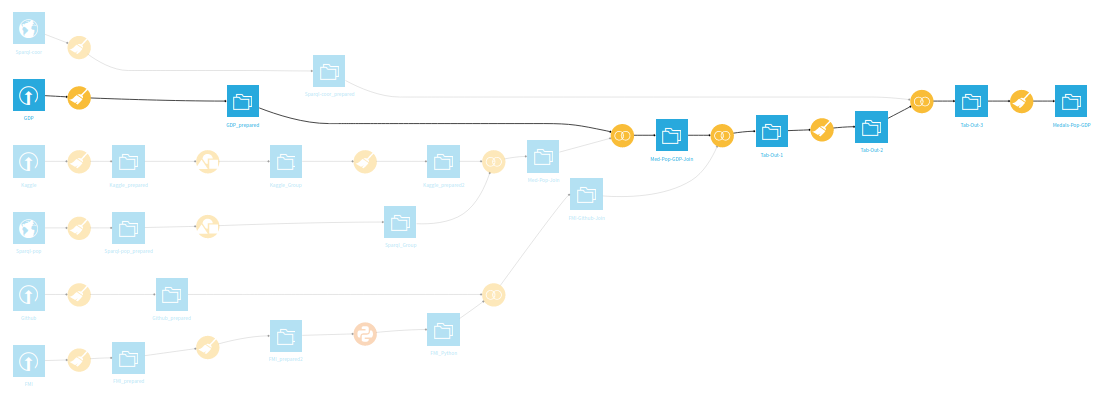
\includegraphics[scale=0.35]{images/flow-medals-gdp.png}
		\caption{Chaîne de traitement du jeu \textit{GDP}}
	\end{figure}
\end{center}

La première recette appliquée est une préparation. Elle consiste en la suppression de toutes les lignes vides -- soit une ligne sur deux -- et la conservation de seulement 7 colonnes sur 68 : \textit{Country Code} pour les codes NOC (fondamentaux pour réaliser de futures jointures) et les 6 colonnes correspondant aux éditions des Jeux Olympiques couvertes par notre travail.

Les colonnes ainsi sélectionnées ont été renommées : \textit{Country Code} devient \textit{NOC} et les colonnes des années suivent le même motif : \textit{1996} devient \textit{1996 - GDP} (pour \textit{Gross Domestic Product}, c'est-à-dire le Produit Intérieur Brut). Enfin, toutes les valeurs décimales ont été arrondies en entier.

Les prochaines étapes du traitement correspondent à des jointures avec d'autres jeux. Nous les détaillerons (\textit{cf}. \textit{infra} p. \pageref{join}) une fois les recettes appliquées à l'ensemble des jeux en amont décrites.





%





\subsection{Préparation du jeu de Kaggle}

Le jeu de Kaggle, nommé \textit{Kaggle} dans Dataiku, correspond à cette partie du flux :

\begin{center}
	\begin{figure}[H]
		\setlength{\belowcaptionskip}{-35pt}
		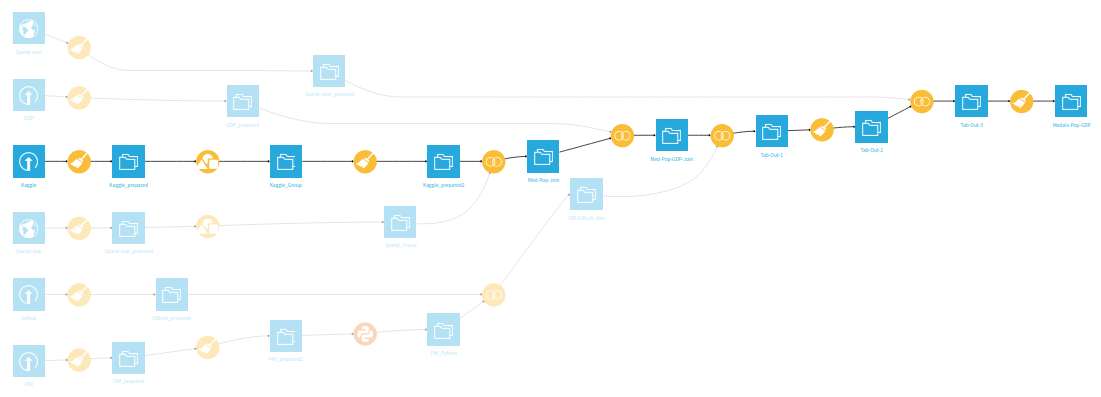
\includegraphics[scale=0.35]{images/flow-medals-kaggle.png}
		\caption{Chaîne de traitement du jeu \textit{Kaggle}}
	\end{figure}
\end{center}

En amont des jointures, ce jeu a fait l'objet de trois recettes. La première, une préparation, nous a permis d'uniquement conserver 3 colonnes sur 15 : \textit{NOC}, \textit{Medal}, \textit{Year}. La colonne \textit{Year} a été épurée pour que seules les années des six éditions deux Jeux y apparaissent. Également, les valeurs nulles de la colonne \textit{Medal} (notées \enquote{N/A}) ont été supprimées.

L'étape suivante consiste en la réalisation d'un pivot. Les années présentes dans les lignes de la colonne \textit{Year} sont devenues des colonnes dont les lignes ont pris pour valeur les entrées de la colonne \textit{Medal}. 6 nouvelles colonnes ont donc été créés, une par édition des Jeux entre 1996 et 2016.

Enfin, nous avons compté les occurrences des trois types de médailles (bronze, argent, or) et créé des colonnes de sortie pour chaque type et pour chaque édition. Par exemple, la colonne \emph{1996} a donné lieu à la création des colonnes \emph{1996 - Bronze} ; \emph{1996 - Silver} ; \emph{1996 - Gold}.

La deuxième recette est un \emph{group}. Le \emph{dataset} présente les médailles reportées par les athlètes, or nous n'avons conservé aucune donnée à leur endroit. Nonobstant, la répartition des médailles repose toujours sur cette logique.

Nous avons donc réalisé un groupement pour réunir les doublons et compter les occurrences de chaque type de médaille remportée pour les six éditions des Jeux. Admettons qu'aux Jeux de 2016, un athlète français ait remporté une médaille de bronze et un autre deux. La recette a pour effet d'afficher le chiffre 3 pour l'entrée \enquote{France} sur la colonne \emph{2016 - Bronze}.

La troisième et dernière recette avant la réalisation des jointures est également une préparation. Elle nous a permis, pour chacune des six éditions, de créer une nouvelle colonne présentant la somme de toutes les médailles remportées par les pays. En guise d'exemple, nous savons qu'à l'édition de 2008, l'Australie a remporté un total de 110 médailles.





%





\subsection{Préparation du jeu de Wikidata (population)}

Le jeu généré grâce à la requête SPARQL sur la population, nommé \textit{Sparql-pop}, correspond à cette partie du flux :

\begin{center}
	\begin{figure}[H]
		\setlength{\belowcaptionskip}{-35pt}
		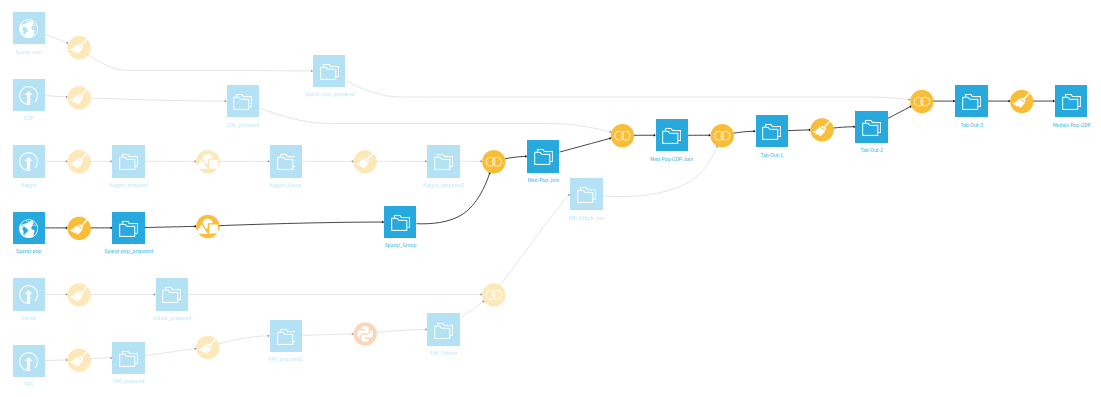
\includegraphics[scale=0.35]{images/flow-medals-sparql-pop.png}
		\caption{Chaîne de traitement du jeu \textit{Sparql-pop}}
	\end{figure}
\end{center}

Ce jeu a été soumis à deux recettes. Une préparation où nous avons supprimé les 8 colonnes dont le suffixe était autre que \enquote{.value} -- lesquelles n'étaient pas sollicitées par notre requête SPARQL (\textit{cf}. \textit{supra} p. \pageref{nongrata}). Trois colonnes ont été renommées : \textit{cio.value} est devenu \textit{NOC} ; \textit{isoCode.value} est devenu \textit{Pays} et \textit{paysLabel.value} est devenu \textit{Nom - Pays}.

Nous avons modifié le format des dates : sur l'année, le jour, le mois et l'horaire, nous n'avons conservé que l'année dans une colonne de sortie avant de supprimer la colonne initiale. Les années des six éditions mises à part, toutes les autres ont été supprimées et un nouveau pivot a été réalisé : les années en ligne sont passées en colonne et ont pris pour valeur le nombre d'habitants par pays. Ce pivot a permis la suppression des colonnes \emph{Année} et \emph{population.value}. Enfin, les colonnes des années ont été renommées selon un motif commun : \emph{1996} est devenu \emph{1996 - Pop}.

La dernière étape de cette recette consiste en la suppression de trois valeurs vides présentes dans la colonne \emph{NOC}.

À l'instar du jeu de Kaggle, nous avons appliqué une recette \emph{group} au jeu de Wikidata. Le groupe s'est effectué sur les colonnes \emph{NOC}, \emph{Pays} et \emph{Nom - Pays} afin de regrouper le nombre d'habitants par année sur une même ligne.





%





\subsection{Préparation du jeu de GitHub}

Le jeu provenant de la plateforme GitHub, nommé \textit{Github} dans Dataiku, correspond à cette partie du flux :

\begin{center}
	\begin{figure}[H]
		\setlength{\belowcaptionskip}{-35pt}
		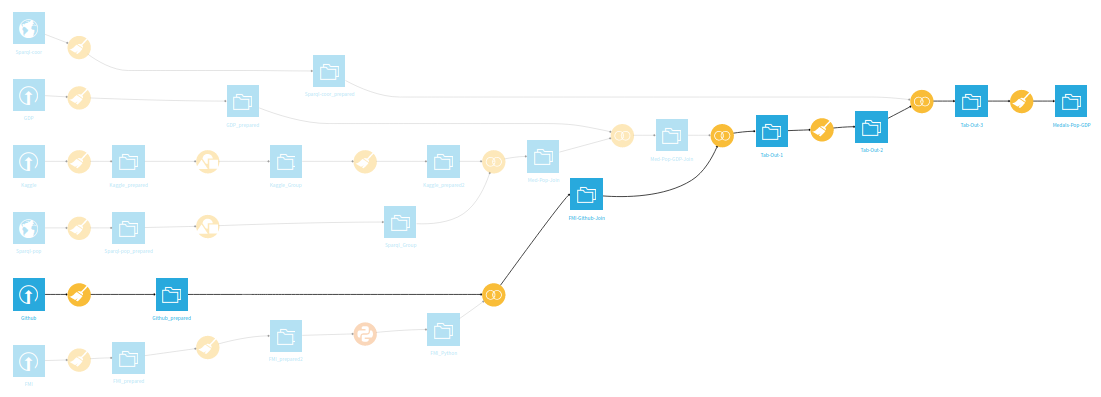
\includegraphics[scale=0.35]{images/flow-medals-github.png}
		\caption{Chaîne de traitement du jeu \textit{Github}}
	\end{figure}
\end{center}

Le jeu n'a nécessité qu'une maigre recette de préparation : nous avons supprimé les colonnes \textit{Alpha-2 Code} et \textit{Numeric Code} pour ne conserver que la colonne \textit{Alpha-3 Code} pour faciliter les jointures.

Nous avons également supprimé les entrées que Dataiku ne reconnaissait pas comme pays. Enfin, nous avons renommé 2 colonnes : \textit{Country} est devenu \textit{Pays} et \textit{Alpha-3 Code} est devenu \textit{Code}.





%





\subsection{Préparation du jeu du FMI}

Le jeu du Fonds Monétaire International, nommé \textit{FMI} dans Dataiku, correspond à cette partie du flux :

\begin{center}
	\begin{figure}[H]
		\setlength{\belowcaptionskip}{-35pt}
		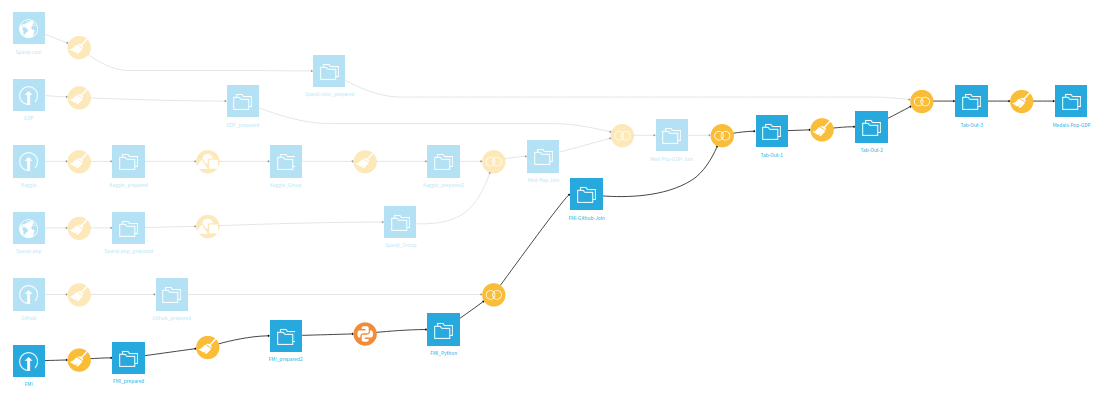
\includegraphics[scale=0.35]{images/flow-medals-fmi.png}
		\caption{Chaîne de traitement du jeu \textit{FMI}}
	\end{figure}
\end{center}

À la faveur de la première recette -- une préparation -- nous avons supprimé de la colonne \textit{Unit Name} les lignes où la valeur était \enquote{Domestic currency} pour ne conserver que le pourcentage du Produit Intérieur Brut (\enquote{Percent of GDP}) investi par les pays dans le domaine du sport.

Nous avons uniquement conservé 7 colonnes : \textit{Country Name} ainsi que les dates des six éditions des Jeux. La dernière étape de la préparation consistait en la suppression de lignes vides pour la colonne \textit{2016}. À partir de ce moment, Dataiku se figeait et nous laissait dans l'impossibilité d'ajouter de nouvelles étapes. Nous avons donc dû ajouter une autre recette de préparation pour que le \textit{run} fonctionne et reprendre le traitement.

Dans cette deuxième préparation, les colonnes des années des Jeux ont été renommées selon le motif suivant : \textit{1996} devient \textit{1996 - FMI}.

Il nous a fallu manuellement modifier 13 valeurs dans la colonne \emph{Country Name} pour une meilleure reconnaissance des pays par Dataiku. Par exemple : \enquote{Russian Federation}, \enquote{Czech Rep.} ne sont pas reconnus, tandis que \enquote{Russia} et \enquote{Czech Republic} le sont. Ces modifications ont donné lieu à la création d'une colonne de sortie \emph{Pays} car il nous était impossible de modifier les noms des pays directement dans la colonne d'origine. Nous avons donc supprimé la colonne \emph{Country Name}, une fois ces modifications effectuées. 

Nous avons rencontré un problème de données aberrantes dans les valeurs indiquées pour les investissements par rapport au PIB. La nature du problème repose sur des conversions mathématiques fautives : les pour mille et pour cent ont subi la même opération. Nous avons donc entrepris de corriger ces données par l'intermédiaire d'une recette Python que voici :

\label{python}\begin{lstlisting}[language=python]
import dataiku
import pandas as pd
from dataiku import pandasutils as pdu

FMI_prepared2 = dataiku.Dataset("FMI_prepared2")
FMI_prepared2_df = FMI_prepared2.get_dataframe()
colonnes_a_traiter = ['1996 - FMI', '2000 - FMI', '2004 - FMI', '2008 - FMI', '2012 - FMI', '2016 - FMI']

for colonne in colonnes_a_traiter:
				condition = FMI_prepared2_df[colonne] > 0.1
				FMI_prepared2_df.loc[condition, colonne] /= 10

FMI_prepared2_df.drop_duplicates(subset=['Pays'], keep='first', inplace=True)
FMI_Python = dataiku.Dataset("FMI_Python")
FMI_Python.write_with_schema(FMI_prepared2_df)
\end{lstlisting}

Le code ci-dessus intervient sur les colonnes des six éditions des Jeux :

\begin{lstlisting}[language=python]	
colonnes_a_traiter = ['1996 - FMI', '2000 - FMI', '2004 - FMI', '2008 - FMI', '2012 - FMI', '2016 - FMI']
\end{lstlisting}

Le contenu de ces colonnes est modifié grâce à une boucle \code{for} : si elles contiennent des valeurs supérieures à \code{0.1}, ces dernières sont divisées par \code{10} pour obtenir la juste valeur d'investissement :

\begin{lstlisting}[language=python]
for colonne in colonnes_a_traiter:
				condition = FMI_prepared2_df[colonne] > 0.1
				FMI_prepared2_df.loc[condition, colonne] /= 10
\end{lstlisting}

Les valeurs deviennent alors cohérentes. Il n'est cependant pas impossible que d'autres problèmes mathématiques émaillent le jeu du FMI mais nous n'avons pu que cerner et traiter celui-ci. 





%





\subsection{Préparation du jeu de Wikidata (coordonnées)}

Rappelons que nous avons dû trouver des données à même de corriger les coordonnées impropres du jeu de GitHub. Ce jeu, également issu d'une requête SPARQL et nommé \textit{Sparql-coor} dans Dataiku, correspond à cette partie du flux :

\begin{center}
	\begin{figure}[H]
		\setlength{\belowcaptionskip}{-35pt}
		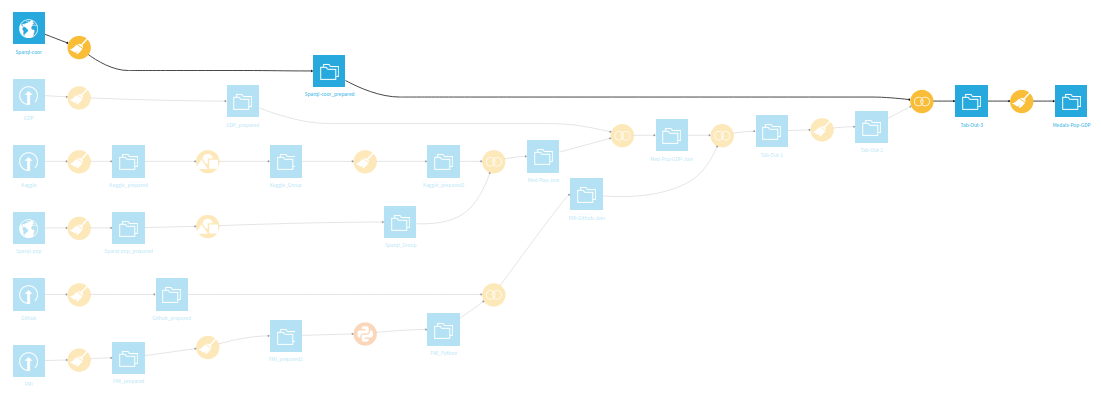
\includegraphics[scale=0.35]{images/flow-medals-sparql-coor.png}
		\caption{Chaîne de traitement du jeu \textit{Sparql-coor}}
	\end{figure}
\end{center}

Une seule recette de préparation a derechef été nécessaire en amont des jointures. Celle-ci ne conserve que les colonnes \textit{noc.value} et \textit{geopoint.value}.

Les deux autres étapes de la recette nous permettent de correctement typer et extraire les coordonnées de la colonne \textit{geopoint.value} afin de correctement les exploiter pour réaliser nos datavisualisations. \label{casse}Les données sont écrites comme suit : \enquote{point(11.0 65.0)}.

Cependant, les données ainsi typées sont effectivement reconnues par le logiciel de datavisualisation Tableau Public comme étant des coordonnées mais équivalent toutes à \enquote{Null} une fois importées.

Nous avons essayé de résoudre le problème directement depuis Tableau Public, sans succès car le logiciel considérait les coordonnées comme des chaînes de caractères et ne pouvait bien entendu pas calculer une longitude et une latitude à partir de ce type de données.

Nous avons finalement compris que le problème était la casse : pour que les données soient correctement typées, il fallait que tous les caractères soient en haut-de-casse : non pas \enquote{point(11.0 65.0)} mais \enquote{POINT(11.0 65.0)}. Nous avons donc ajouté cette étape dans la recette avant d'extraire les longitudes et latitudes dans 2 colonnes distinctes.





%





\label{join}\subsection{Première jointure}

La première jointure concerne les jeux préparés \textit{Kaggle} et \textit{Sparql-pop}, selon la colonne \textit{NOC}. Il en résulte la création du jeu \textit{Med-Pop-Join}, lequel contient 33 colonnes. 2 colonnes sur le code des pays, 1 sur leur nom, 6 colonnes sur la population des années correspondant aux éditions des Jeux et 4 colonnes par année : 3 pour les types de médailles et 1 pour la somme de ces dernières.

Cette \textit{left join} s'est réalisée sans suppression et n'a pas occasionné de pertes significatives de données.





%





\subsection{Deuxième jointure}

À la suite de cette première jointure s'effectue une deuxième \textit{left join} : les jeux \textit{Med-Pop-Join} et \textit{GDP} sont ainsi regroupés -- également selon la colonne \textit{NOC} -- engendrant le jeu \textit{Med-Pop-GDP-Join}. 6 colonnes ont été alors ajoutées aux 33 du jeu \textit{Med-Pop-Join}. Elles correspondent au PIB des pays pour chaque année d'édition des Jeux Olympiques.





%





\subsection{Troisième jointure}

Une troisième \textit{left join} croise les jeux \textit{FMI} et \textit{Github}, selon la colonne \textit{Pays} du jeu \textit{FMI}. Le jeu \textit{FMI-Github-Join} est créé et contient 10 colonnes. Les données du Fonds Monétaire International ont ainsi été enrichies par le code et les coordonnées des pays, fournies par le jeu de GitHub.





%





\subsection{Quatrième jointure}

La quatrième jointure rassemble les jeux \textit{Med-Pop-GDP-Join} et \textit{FMI-Github-Join}. Dans la mesure où les médailles remportées constituent les données les plus importantes à nos yeux, la \textit{left join} a été réalisée de telle sorte à ce que les pertes, s'il devait y en avoir, aient des conséquences sur les données du jeu \textit{FMI-Github-Join} -- non pas sur celles du jeu \textit{Med-Pop-GDP-Join}.





%





\subsection{Préparation du jeu final}

Le jeu créé, nommé \textit{Tab-Out-1} a subi une recette de préparation afin de nettoyer (nous le pensions) une dernière fois les données. \label{orga}42 de ses 47 colonnes ont été réorganisées selon un même schéma pour chaque édition des Jeux :

\begin{center}
	\begin{figure}[H]
		\centering
		\setlength{\belowcaptionskip}{-35pt}
		
\includegraphics[scale=0.5]{images/tab-out.png}
		\caption{Extrait du jeu \textit{Tab-Out-1}}
	\end{figure}
\end{center}

Les 5 autres colonnes présentent le nom des pays, leurs codes et leurs coordonnées. Nous pensions que ce jeu ainsi nettoyé, nommé \textit{Tab-Out-2}, était la dernière étape du flux. Cependant, une fois importé dans Tableau Public, les coordonnées se sont révélées inutilisables. C'est pourquoi la seconde requête SPARQL sur les coordonnées des pays était nécessaire. 

Nous avons donc réalisé une dernière jointure sur les jeux \textit{Sparql-coor} et \textit{Tab-Out-2}. Il s'agit d'une \textit{inner join} selon le code NOC. Le jeu alors créé, \textit{Tab-Out-3} voit ses valeurs de coordonnées corrigées.

Ce jeu de sortie a fait l'objet d'un dernier nettoyage tardif. D'une part, la colonne \textit{2004 - GDP} avait échappé à l'étape d'organisation précédemment décrite (\textit{cf}. \textit{supra} p. \pageref{orga}). D'autre part, nous ne suivions pas un mode de nommage de colonnes tout à fait rigoureux. Comme nous avions prévu de présenter des données en langue anglaise, nous avons renommé toutes les colonnes dont tout ou partie de l'intitulé était encore en français.

Est créé notre jeu final : \textit{Medals-Pop-GDP}, au terme du flux ci-dessous.

\begin{center}
	\begin{figure}[H]
		\centering
		\setlength{\belowcaptionskip}{-35pt}
		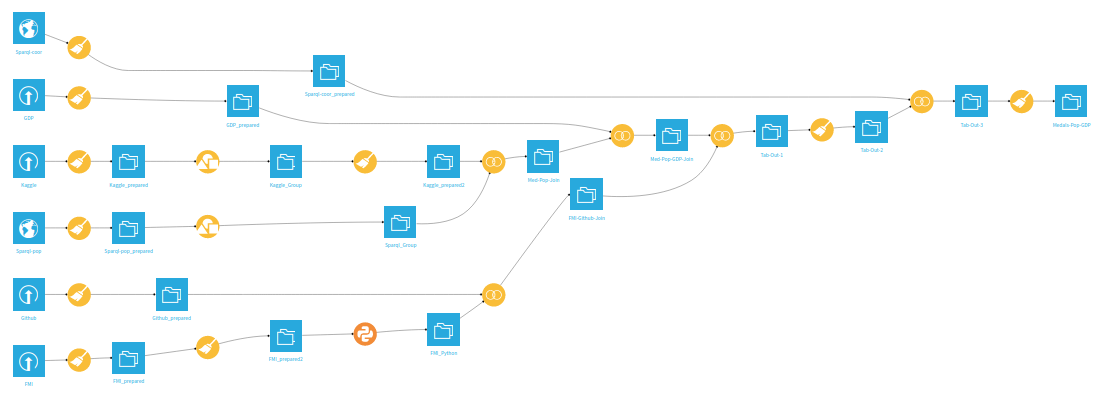
\includegraphics[scale=0.35]{images/flow-medals-full.png}
		\caption{Flux de traitement sur les médailles et les investissements}
	\end{figure}
\end{center}





%





\section{Chaîne de traitement du second flux}

Notons que ce deuxième flux est composé de trois petits flux qu'il ne fait pas sens de joindre en bout de chaîne sur Dataiku. La mise en relation des quatre jeux de données finaux sera l'objet des datavisualisations.

Le premier mini-flux a pour sujet les infrastructures relatives à la natation du Royaume-Uni, \textit{idem} pour le deuxième mini-flux à l'égard de la France et le troisième concerne les médailles remportées par les deux pays.

Par souci de concision et de clarté à l'égard des intitulés des différentes étapes, nous avons fait le choix de trois entêtes distincts : \enquote{GBR} pour le mini-flux sur le Royaume-Uni, \enquote{FRA} pour le mini-flux sur la France et \enquote{MED} pour le mini-flux sur les médailles remportées par les deux pays aux épreuves de natation des Jeux.





%





\subsection{GBR : préparation des jeux de \textit{Sport England}}

Les jeux \textit{Swimming-Pools} et \textit{Geographic} ont tous deux été préparés en amont de leur jointure. Ils correspondent à cette partie du flux général :

\begin{center}
	\begin{figure}[H]
		\centering
		\setlength{\belowcaptionskip}{-35pt}
		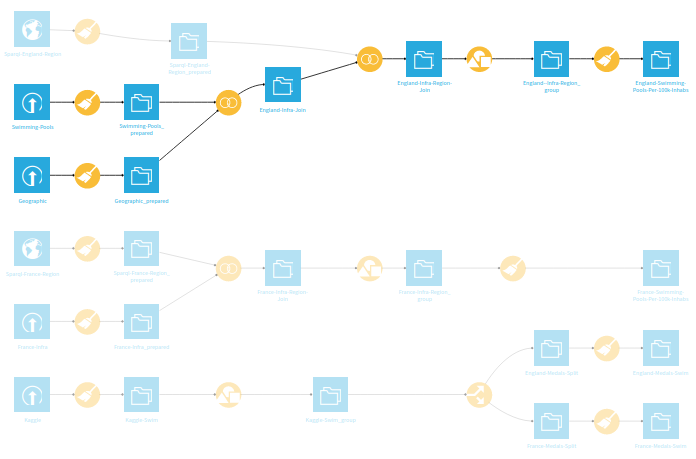
\includegraphics[scale=0.5]{images/flow-swim-eng-sport.png}
		\caption{Chaîne de traitement des jeux \textit{Swimming-Pools} et \textit{Geographic}}
	\end{figure}
\end{center}

Du jeu \textit{Swimming-Pools} n'a été gardée que la colonne \textit{FacilityID} -- précisément pour réaliser une jointure avec le jeu \textit{Geographic}. Dans la mesure où chaque identifiant unique d'infrastructure compte pour 1, nous n'avons besoin d'aucune autre colonne pour la suite du traitement.

Un processus similaire de sélection a été appliqué au jeu \textit{Geographic} : nous n'avons conservé que 4 colonnes, \textit{FACILITYID}, \textit{Region Name}, \textit{Latitude}, \textit{Longitude}. La présence des identifiants uniques dans les deux jeux nous a permis de réaliser une jointure interne et ainsi de lier les infrastructures de natation aux régions d'Angleterre, dans le jeu \textit{England-Infra-Join} nouvellement créé.





%





\subsection{GBR : préparation du jeu de Wikidata}

La requête SPARQL, ici nommée \textit{Sparql-England-Region}, correspond à cette partie du flux :

\begin{center}
	\begin{figure}[H]
		\centering
		\setlength{\belowcaptionskip}{-35pt}
		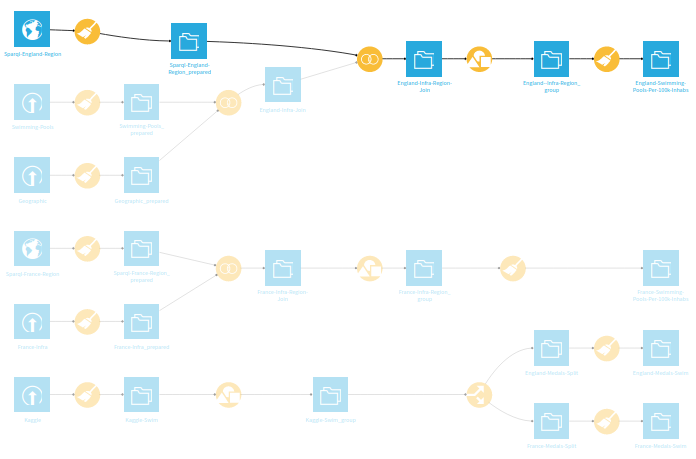
\includegraphics[scale=0.5]{images/flow-swim-eng-sparql.png}
		\caption{Chaîne de traitement du jeu \textit{Sparql-England-Region}}
	\end{figure}
\end{center}

Avant de réaliser la jointure avec les deux autres jeux de ce mini-flux, nous appliquons une recette de préparation à celui-ci. Des colonnes initiales, nous n'en conservons que 3 : \textit{population.value}, \textit{geopoint.value} et \textit{RegionLabel.value} -- soit le nombre d'habitants des régions, leurs coordonnées et leur nom.

Nous évacuons les lignes vides de la colonne \textit{population.value} et renommons manuellement certaines données de la colonne \textit{RegionLabel.value} pour une meilleure reconnaissance, à la fois par Dataiku et Tableau Public. Pour que les coordonnées soient reconnues et exploitables (\textit{cf}. \textit{supra} p. \pageref{casse}), nous convertissons toutes les valeurs textuelles de la colonne \textit{geopoint.value} en haut-de-casse. Enfin, nous extrayons les valeurs de longitude et de latitude de cette même colonne et créons ainsi les colonnes \textit{Latitude} et \textit{Longitude}.





%





\subsection{GBR : jointure et préparation du jeu final}

La jointure interne des jeux \textit{Sparql-England-Region} et \textit{England-Infra-Join} a été effectuée sur le nom des régions. Il en ressort le jeu \textit{England-Infra-Region-Join}, composé de 5 colonnes : le nom, les coordonnées, la population des régions et l'identifiant des infrastructures.

Nous avons appliqué une recette de groupement sur ce jeu, selon les colonnes \textit{population.value} et \textit{FacilityID} pour n'avoir qu'une ligne par région et par nombre d'habitants. De ce fait, la colonne \textit{FacilityID} a donné lieu à la nouvelle colonne \textit{count}, laquelle présente la somme des infrastructures par région. Cette donnée est au cœur de la dernière recette. Celle-ci nous permet, par l'intermédiaire d'un produit en croix, de compter le nombre d'infrastructure par région pour 100.000 habitants et de l'afficher dans la colonne \textit{Swimming pools per 100k inhabitants}. Notre jeu final, \textit{England-Swimming-Pools-Per-100k-Inhabs} est ainsi créé.





%





\subsection{FRA : préparation du jeu du ministère}

Le jeu du ministère (\textit{France-Infra}), à l'instar du jeu de Wikidata sur les régions françaises, a été préparé avant la jointure nécessaire. Il correspond à cette partie du flux :

\begin{center}
	\begin{figure}[H]
		\centering
		\setlength{\belowcaptionskip}{-35pt}
		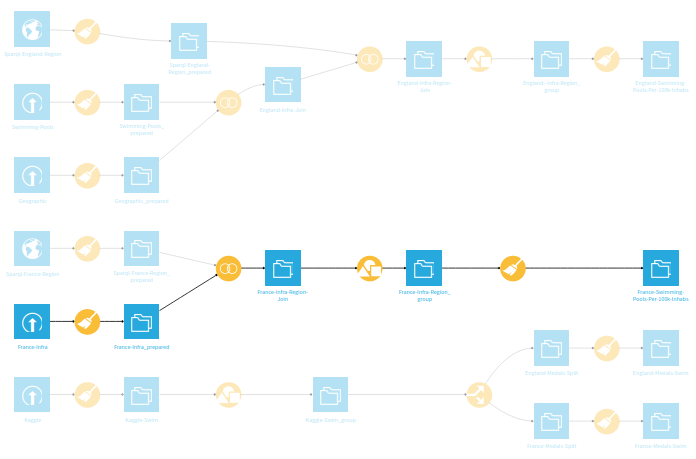
\includegraphics[scale=0.5]{images/flow-swim-fra-ministere.png}
		\caption{Chaîne de traitement du jeu \textit{France-Infra}}
	\end{figure}
\end{center}

Seules 4 colonnes ont été conservées : \textit{Type d'équipement sportif}, \textit{Longitude (WGS84)}, \textit{Latitude (WGS84)} et \textit{Région Nom}. Nous avons ensuite examiné plus en détails les lignes de la colonne \textit{Type d'équipement sportif} et avons pu établir une liste de 5 valeurs relatives à la natation. Nous avons supprimé toutes les lignes qui n'y correspondaient pas. Ces valeurs ont été communément renommées \enquote{picisines\_centres\_aquatiques}.





%





\subsection{FRA : préparation du jeu de Wikidata}

Le jeu de Wikidata sur les régions de France, nommé \textit{Sparql-Region-France} correspond à cette partie du flux :

\begin{center}
	\begin{figure}[H]
		\centering
		\setlength{\belowcaptionskip}{-35pt}
		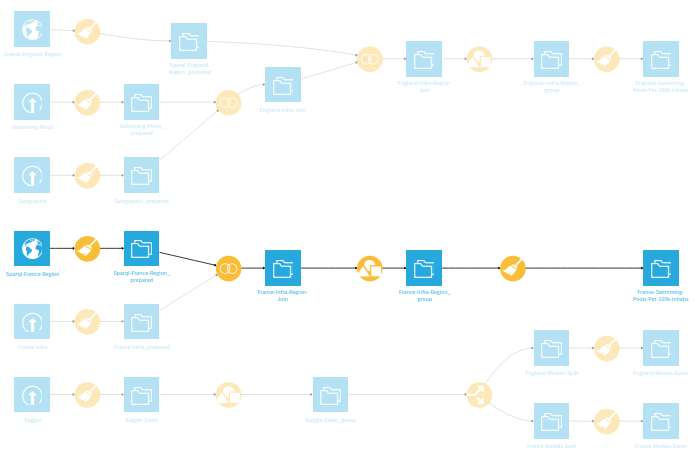
\includegraphics[scale=0.5]{images/flow-swim-fra-sparql.png}
		\caption{Chaîne de traitement du jeu \textit{Sparql-Region-France}}
	\end{figure}
\end{center}

Seules les colonnes \textit{population.value}, \textit{geopoint.value} et \textit{RegionLabel.value} ont été conservées et renommées. De la même manière que pour le jeu Wikidata sur les régions d'Angleterre, les lignes de la colonne \textit{geopoint.value} ont été mises en haut-de-casse, les longitudes et latitudes extraites dans deux nouvelles colonnes, \textit{Longitude}, \textit{Latitude}.





%





\subsection{FRA : jointure et préparation du jeu final}

La jointure interne des jeux \textit{France-Infra} et \textit{Sparql-France-Region} a été réalisée selon la colonne des noms de région. Le jeu ainsi créé, \textit{France-Infra-Region-Join} est tout à fait similaire au jeu \textit{England-Infra-Region-Join}. Les dernières recettes sont \textit{de facto} analogues.

Nous réalisons un groupement sur les types d'équipement et effectuons derechef un produit en croix pour générer une colonne \textit{Swimming pools per 100k inhabitants}. Le dernier jeu de ce mini-flux, nommé \textit{France-Swimming-Pools-Per-100k-Inhabitants} émerge alors. 





%





\subsection{MED : préparation du jeu de Kaggle}

Enfin, le jeu \textit{Kaggle} issu de notre premier flux (précisément du jeu nommé \textit{Kaggle\_prepared2}) correspond à cette partie de la chaîne :

\begin{center}
	\begin{figure}[H]
		\centering
		\setlength{\belowcaptionskip}{-35pt}
		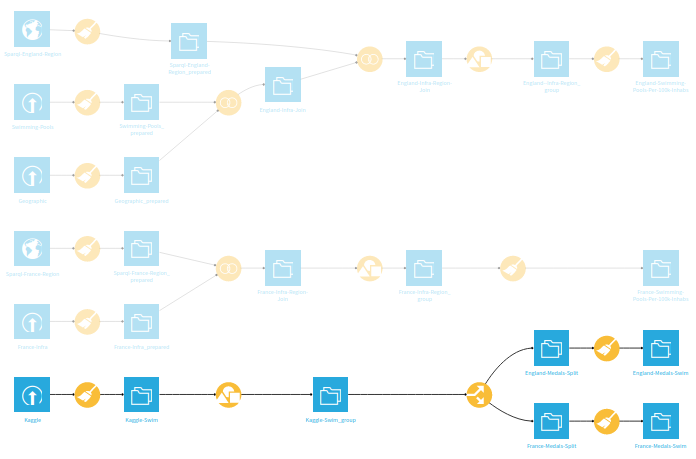
\includegraphics[scale=0.5]{images/flow-swim-kaggle.png}
		\caption{Chaîne de traitement du jeu \textit{Kaggle}}
	\end{figure}
\end{center}

Dans une première recette de préparation, nous avons identifié les lignes de la colonne \textit{Sport} relatives à la natation, les avons renommées \enquote{Swimming\_sports} et avons supprimé toutes les autres. Également, nous n'avons conservé que les lignes où le code NOC est équivalent à \enquote{FRA} et \enquote{GBR}.

Nous avons ensuite appliqué une recette de groupement pour que seules 2 lignes affichent l'ensemble des médailles remportées, d'une part par la France, d'autre part par le Royaume-Uni. L'avant-dernière recette sépare le jeu groupé en deux jeux distincts : l'un pour les médailles remportées par la France, l'autre pour les médailles remportées par le Royaume-Uni.

\subsection{MED : préparation du jeu final}

Les deux jeux alors créés, \textit{England-Medals-Split} et \textit{France-Medals-Split} ont été identiquement nettoyés : la langue et la casse des noms de colonnes harmonisées et leur ordre basé sur le même motif que celui adopté pour le jeu du premier flux (\textit{cf}. \textit{supra} p. \pageref{orga}). Nos deux jeux finaux, \textit{England-Medals-Swim} et \textit{France-Medals-Swim} closent la chaîne de traitement de ce mini-flux.

Notre deuxième grand flux a donc abouti à la création de quatre jeux de données, lesquels seront tous exploités et liés dans nos datavisualisations :

\begin{center}
	\begin{figure}[H]
		\centering
		\setlength{\belowcaptionskip}{-35pt}
		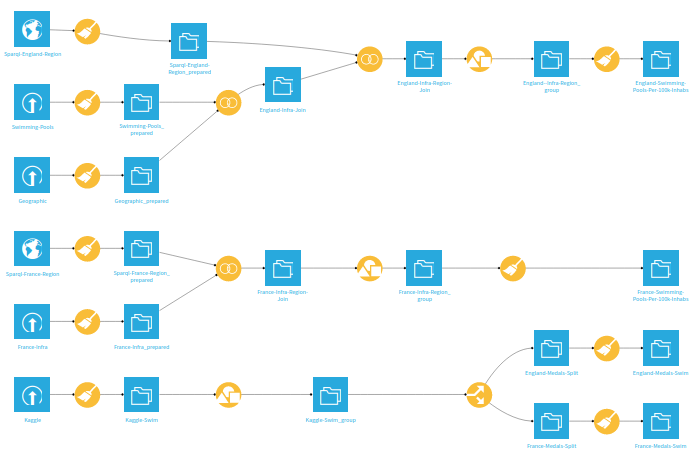
\includegraphics[scale=0.5]{images/flow-swim-full.png}
		\caption{Flux de traitement sur les médailles de natation}
	\end{figure}
\end{center}





%





\chapter{Visualisation des données}

À l'aune de nos différents jeux de sortie et de notre approche en deux temps, nous avons produit un ensemble de six datavisualisations.

Trois ont été créées à partir du premier flux de données, soit le nombre de médailles remportées par les pays sur six éditions des Jeux Olympiques au regard de leur PIB, de leur niveau d'investissement dans le domaine sportif et de leur nombre d'habitants. Ces visualisations-ci ont donné lieu à la composition d'une \enquote{histoire}\autocite{vismap}.

Trois autres visualisations exploitent les données de notre deuxième grand flux, lui-même composé -- rappelons-le -- de trois petits flux. Elles mettent en relief le nombre de médailles remportées par la France et l'Angleterre pour les épreuves de natation au regard du nombre d'infrastructures sportives relatives par région et pour 100.000 habitants. Ces visualisations ont donné lieu à la création d'un tableau de bord\autocite{visswim}.

\section{Visualisations du premier flux}

\subsection{Médailles remportées par les pays : carte du monde}

\label{map}Notre première visualisation adopte le format d'une carte du monde :

\begin{center}
	\begin{figure}[H]
		\centering
		\setlength{\belowcaptionskip}{-35pt}
		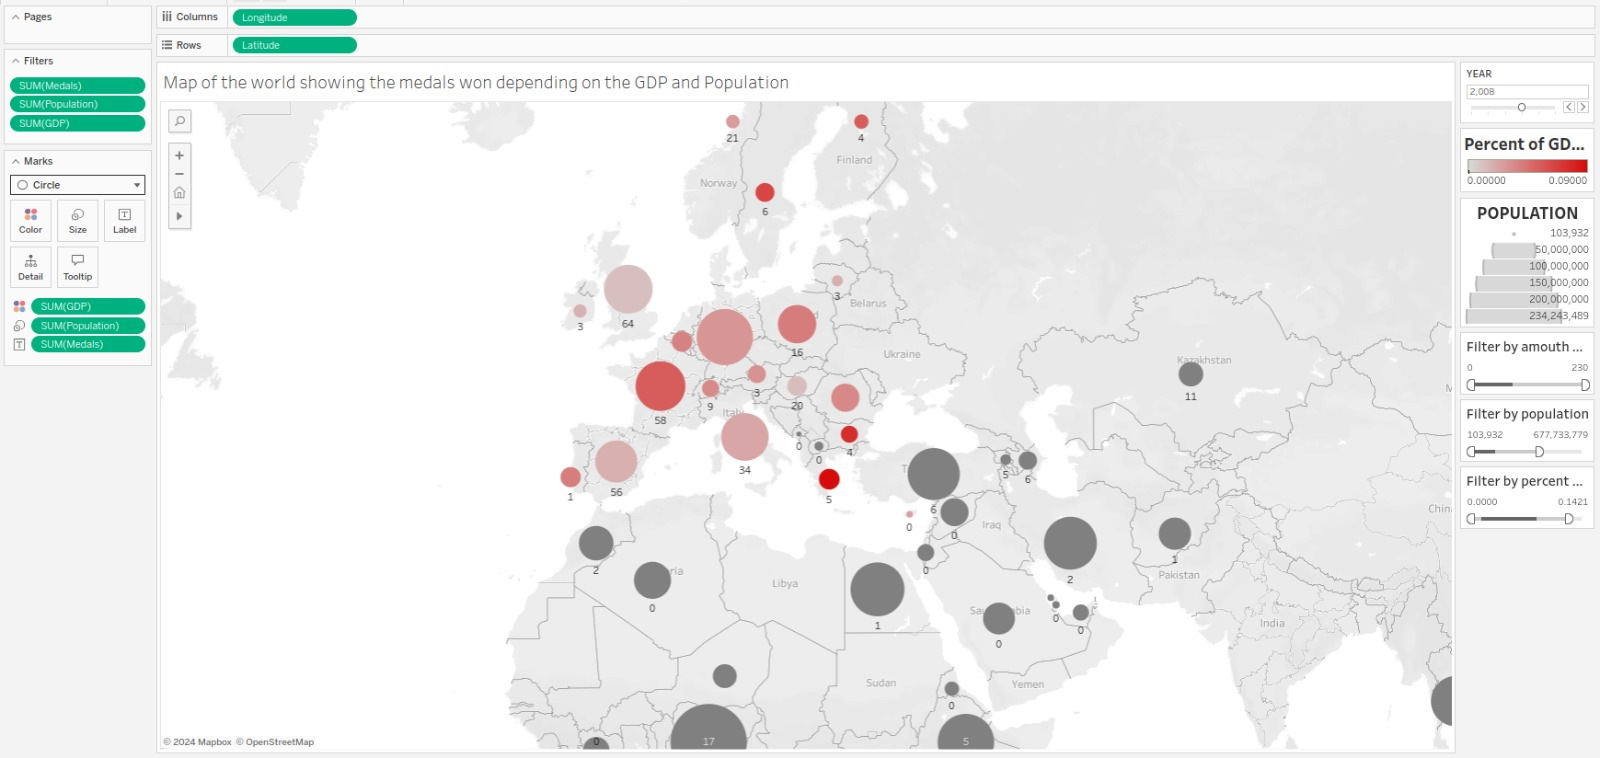
\includegraphics[scale=0.25]{images/datavis-medals-world-map.jpeg}
		\captionsetup{justification=centering}
		\caption{Aperçu de la visualisation \textit{Map of the world showing the medals won depending on the GDP and Population} (année 2008)}
	\end{figure}
\end{center}

\subsubsection{Ambition de la visualisation}

Son but est de montrer le lien entre population, richesse -- matérialisée par le Produit Intérieur Brut -- et le nombre de médailles remportées à six éditions des Jeux. L'utilisateur peut naviguer entre les différentes années (1996, 2000, 2004, 2008, 2012 et 2016) en manipulant une liste déroulante et sélectionner l'année de son choix. Afin d'afficher au mieux ces trois paramètres (médailles, population, investissements), il nous a semblé pertinent de combiner différentes sortes d'indices visuels.

Le nombre de médailles est présenté sous forme d'étiquette (voyez sur l'image ci-dessus, \enquote{58} pour la France ou \enquote{1} pour le Portugal).

\label{color}Le pourcentage des dépenses dans le sport par rapport au PIB (noté \enquote{GDP}) apparaît selon une échelle de couleurs. Nous avons pris soin de modifier la valeur \textit{center} (\textit{cf}. figure \ref{param} \textit{infra} p. \pageref{param}) pour que les valeurs égales à zéro (incluant les valeurs nulles interprétées par Tableau Public comme tel) apparaissent en gris foncé. \textit{A contrario}, l'échelle de couleur pour les valeurs non nulles et non égales à zéro va du blanc au rouge. 

Nous avons également défini la valeur maximale du PIB investi à 0.09 \%. Aucun pays n'investit plus que 0.1 \% de son PIB dans le domaine sportif, les données contraires présentes dans le jeu du FMI relèvent d'erreurs de saisies que notre formule Python n'a pas été en mesure de corriger (\textit{cf}. \textit{supra} p. \pageref{python}). 

Enfin, la population prend la forme de \enquote{bulles} couvrant tout ou partie du pays concerné. Plus une bulle est grande, plus un pays est fortement peuplé. Les valeurs nulles et égales à zéro sont malgré tout visibles (documentées en légende de la visualisation) sous la forme de points à la taille très réduite.

\begin{center}
	\begin{figure}[H]
		\centering
		\setlength{\belowcaptionskip}{-35pt}
		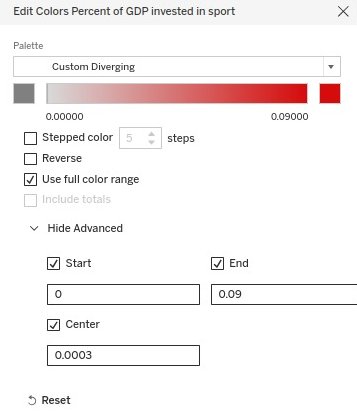
\includegraphics[scale=0.5]{images/datavis-medals-world-center.png}
		\caption{Aperçu d'un paramètre de visualisation sur Tableau Public}
		\label{param}
	\end{figure}
\end{center}

\subsubsection{Difficultés rencontrées}

Si l'on met de côté l'évident problème de manque de données pour certains pays en dépit de notre traitement, nous avons été confrontés à deux obstacles majeurs au cours de la réalisation de cette visualisation.

Le premier concerne l'utilisation de valeurs géographiques dans Tableau Public. Nos données de coordonnées étaient exprimées, dans nos différents jeux, comme ceci \enquote{POINT(56,00 -75,24)}. Dataiku reconnaissait bien leur caractère géographique -- à l'inverse de Tableau Public. Il nous générait effectivement des latitudes et les longitudes mais considérait les données comme des chaînes de caractères et tentait donc de leur appliquer des calculs pour en extraire des coordonnées -- ce qui n'avait aucune chance d'aboutir.

Nous avons donc dû contourner le problème en extrayant nous-mêmes les longitudes et latitudes dans des colonnes dédiées au sein de Dataiku afin de pouvoir les exploiter dans Tableau Public (\textit{cf}. \textit{supra} p. \pageref{casse}).

La deuxième difficulté a été plus complexe à appréhender. Nous souhaitions absolument rendre possible la navigation entre les différentes années. Cependant, notre format de données ne le permettait pas, car il aurait fallu une colonne \textit{Année} sur laquelle nous aurions pu appliquer un filtre.

Pour ce faire, nous aurions pu réaliser un pivot (Tableau Public propose cette fonctionnalité) mais cela aurait gravement perturbé la forme d'autres données que nous ne pouvions pas soumettre à une telle manipulation (latitude, longitude, codes des pays). Nous avons alors consulté la documentation et élaboré beaucoup de tests infructueux pour finalement comprendre que nous devions procéder en deux temps.

Il nous fallait d'abord créer un paramètre nommé \code{YEAR} avec pour valeur les années que nous souhaitons afficher puis créer des champs calculés (à insérer en lieu et place des années) comme ceci :

\begin{lstlisting}[language=tableau]
	IF [YEAR] == 1996 THEN [1996 - Medals]
		ELSEIF [YEAR] == 2000 THEN [2000 - Medals]
		ELSEIF [YEAR] == 2004 THEN [2004 - Medals]
		ELSEIF [YEAR] == 2008 THEN [2008 - Medals]
		ELSEIF [YEAR] == 2012 THEN [2012 - Medals]
		ELSEIF [YEAR] == 2016 THEN [2016 - Medals]
	END
\end{lstlisting}

Ainsi, en fonction de l'année sélectionnée dans la liste \code{YEAR}, le paramètre relatif aux médailles change en conséquence. Nous avons procédé identiquement pour les investissements et la population. Ainsi, quand l'utilisateur sélectionne une année, les données s'actualisent en un instant.

\subsubsection{Regard critique et biais}

Nous avons identifié un ensemble de quatre biais. En première instance, les modes de représentation que nous avons à notre disposition sur Tableau Public font ressortir les problèmes de manque de données. Si le pourcentage d'investissement d'un pays est non-nul mais que sa population n'est pas renseignée, la couleur de la bulle sera tout à fait difficile à cerner. Ce cas de figure est fort heureusement très rare car nos données sur les investissements sont très souvent concomitantes avec nos données sur la population, et \textit{vice-versa}.

Un deuxième biais particulièrement visible est dû au cruel manque de données pour les nations hors pays du premier monde (le jeu du FMI et les résultats des requêtes SPARQL n'étaient que peu éloquents à leur endroit). Par voie de conséquence, il est difficile de tirer des conclusions hors continent européen à la seule consultation de la visualisation.

Le troisième biais se traduit par une espèce de surcharge d'informations directement liée à l'approche de notre travail. Nous avons ici mis en relief trois dimensions : investissements, population et nombre de médailles remportées, sur des espaces géographiques réduits (en l'occurrence, les frontières des pays). Cet effet de surcharge est d'autant plus fort à cause de la diversité des visualisations (étiquettes chiffrée, couleurs, bulles).

Cet état de fait peut demander un certain effort à l'utilisateur pour correctement identifier les données et leur mode de représentation. Pour réduire ce biais au maximum, nous avons proposé une légende détaillée de notre visualisation avec une mise à disposition de différents filtres pour que l'affichage des données puisse être manipulé et adapté.

Le quatrième et dernier biais concerne la lisibilité des évolutions d'une édition des Jeux Olympiques à l'autre car nous ne proposons pas un affichage simultané de plusieurs années. Il est donc plus corsé, en première lecture, de visuellement constater si l'évolution des investissements d'un pays suit l'évolution du nombre de médailles gagnées ou non.

Nous maintenons notre choix de visualisation et de sélection libre de l'année représentée -- avant tout pour des questions de commodité de lecture en cherchant à surcharger au minium la carte.





%





\subsection{Médailles remportées par les pays : histogramme}

Notre deuxième visualisation est un diagramme en barres empilées :

\begin{center}
	\begin{figure}[H]
		\setlength{\belowcaptionskip}{-35pt}
		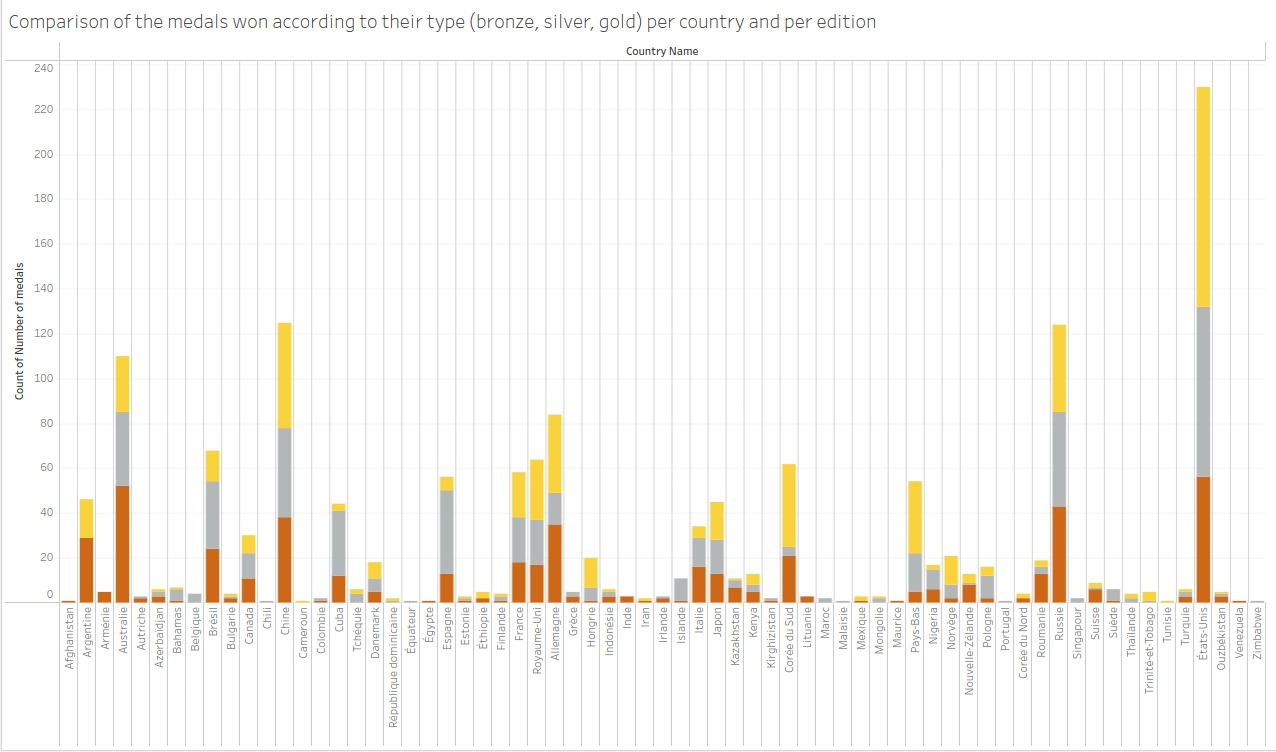
\includegraphics[scale=0.3]{images/datavis-medals-world-histo.jpeg}
		\captionsetup{justification=centering}
		\caption{Aperçu de la visualisation \textit{Comparison of the medals won according to their type (bronze, silver, gold) per country and per edition}}
	\end{figure}
\end{center}

\subsubsection{Ambition de la visualisation}

Cette deuxième visualisation vise en premier lieu à présenter l'évolution du nombre de médailles remportées par tous les pays participants aux Jeux entre 1996 et 2016. Si elle ne comporte ni donnée économique ni donnée géographique, elle est à considérer comme un complément de notre première visualisation (\textit{cf}. \textit{supra} p. \pageref{map}) dans la mesure où elle détaille le rang des médailles remportées par les pays : bronze, argent ou or.

Pour ce faire, la visualisation présente en abscisse le nom des pays et en ordonnée, le nombre de médailles. Le survol des barres avec le curseur détaille les informations -- que nous avons voulu synthétiser visuellement grâce à un choix adéquat de couleurs : doré pour les médailles d'or, gris pour les médailles d'argent et brun pour les médailles de bronze.

Nous avons voulu cette visualisation simple et facilement compréhensible pour les utilisateurs désireux de la consulter en parallèle de la carte et de mieux saisir la répartition des médailles selon l'édition sélectionnée. C'est pourquoi nous avons soumis les deux visualisations au même paramètre de choix pour que l'ensemble des données s'actualise en même temps.

\subsubsection{Difficultés rencontrées}

La grande difficulté concernait derechef le format de nos données. Nous pensions qu'avec des colonnes \textit{Bronze}, \textit{Silver} et \textit{Gold} distinctes, nous aurions pu les exploiter pour générer un diagramme en barres empilées. De nouveau, consulter la documentation nous a fait réaliser que pour ce mode de visualisation, nous devions avoir -- en lieu et place des nombres de médailles gagnées dans chaque colonne -- des colonnes avec autant d'occurrences de \enquote{bronze}, \enquote{silver} et \enquote{gold} que de pays ayant gagné les médailles.

\subsubsection{Regard critique et biais}

Mis à part une consultation des données plus difficile au survol de la souris pour les pays ayant gagné le moins de médailles -- en raison de la petitesse de leur barre -- nous ne constatons pas de biais à l'égard de cette visualisation. 





%





\subsection{PIB et investissements : carte à cases}

Notre troisième et dernière visualisation prend la forme d'une carte à cases, également nommée \textit{treemap} :

\begin{center}
	\begin{figure}[H]
		\centering
		\setlength{\belowcaptionskip}{-35pt}
		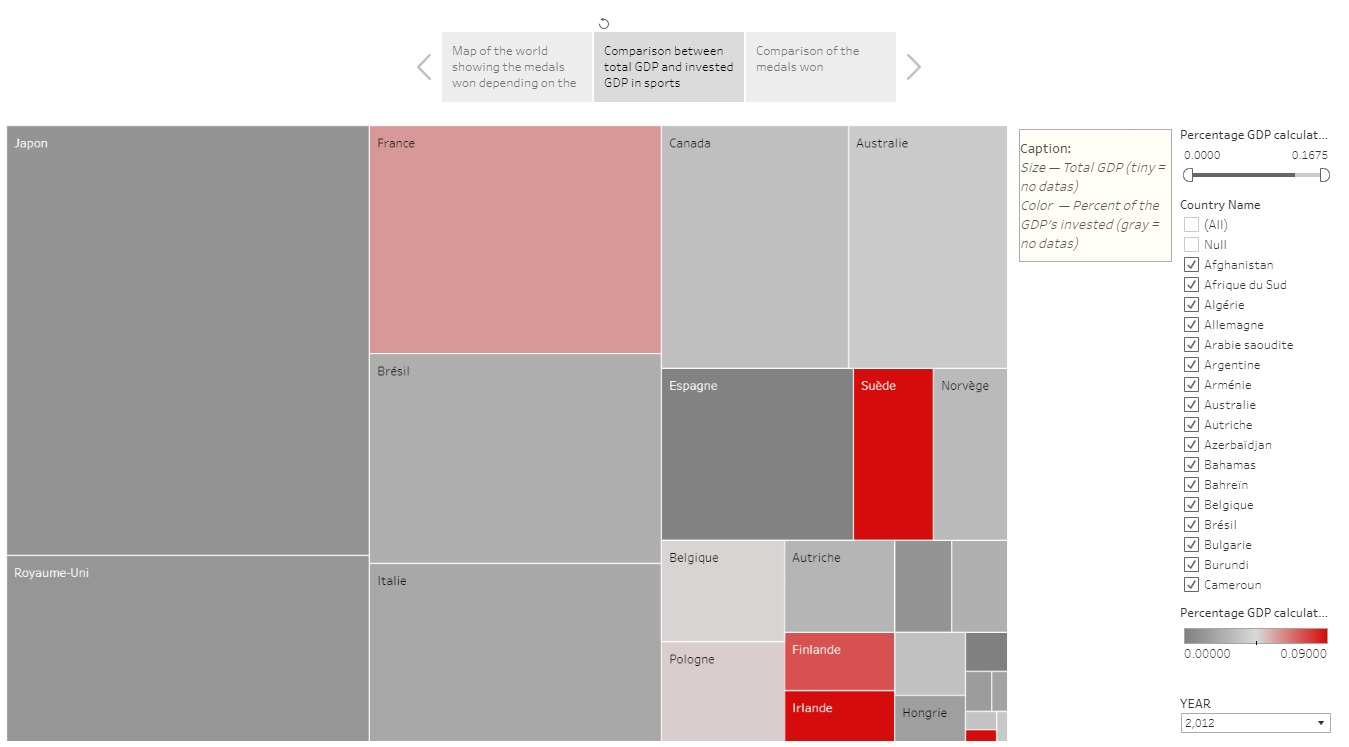
\includegraphics[scale=0.25]{images/datavis-medals-world-treemap.jpeg}
		\captionsetup{justification=centering}
		\caption{Aperçu de la visualisation \textit{Comparison between total GDP and invested GDP in sports} (année 2000)}
	\end{figure}
\end{center}

\subsubsection{Ambition de la visualisation}

Son but est de venir à la rescousse de notre visualisation en carte du monde, laquelle montre le pourcentage du Produit Intérieur Brut investi par les pays sans pour autant fournir les chiffres du PIB. Or si la Russie et les États-Unis investissent tous deux 0.05\% de leur PIB dans le domaine sportif, il ne faut certainement pas songer à un niveau d'investissement et de répartition des infrastructures comparables.

Ainsi, cette carte à case indique le PIB total des pays selon une échelle de taille et son pourcentage investi dans le sport selon une échelle de couleur (identique à celle utilisée pour la carte du monde, \textit{cf}. \textit{supra} p. \pageref{color}), plus le pourcentage d'investissement est fort, plus le pays apparaîtra en rouge. Également, l'utilisateur peut -- selon le même paramètre établi pour les deux autres visualisations -- changer l'année à sa guise et choisir parmi les six éditions des Jeux Olympiques. Il est également possible de sélectionner les pays que l'on souhaite afficher par l'intermédiaire d'une liste à cocher.

\subsubsection{Difficultés rencontrées}

L'aisance acquise lors de la conception des premières visualisations nous a fait faire l'économie de difficultés à propos de celle-ci.

\subsubsection{Regard critique et biais}

Nous pouvons soulever le manque d'une troisième donnée -- en l'occurrence, la population -- laquelle aurait pu consolider la visualisation. L'utilisateur aurait ainsi eu un regard sur les investissements dans le sport selon le pourcentage du PIB et la population. Néanmoins, dans le temps qui nous était imparti, nous n'avons pu trouver une manière saillante et consistante de représenter autant de données dans un modèle de la sorte.

Notons également le manque de données à l'origine de nombreux déséquilibres visuels dans la visualisation. Comme indiqué en légende, les pays dont nous ne connaissons pas le montant du PIB sont relégués aux plus petites tailles et les pays dont nous ne connaissons pas le pourcentage investi dans le domaine sportif apparaissent en gris foncé. C'est pourquoi nous avons mis à disposition des options de tri afin d'adapter au mieux l'affichage des données.
\newline

Précisons enfin que cette visualisation a été très tardivement réalisée. Nous voulions exploiter les données relatives au montant du PIB sans perturber notre tableau de bord, or aucun essai n'a porté ses fruits. En voici un aperçu avant l'intégration de cette troisième visualisation :

\begin{center}
	\begin{figure}[H]
		\centering
		\setlength{\belowcaptionskip}{-35pt}
		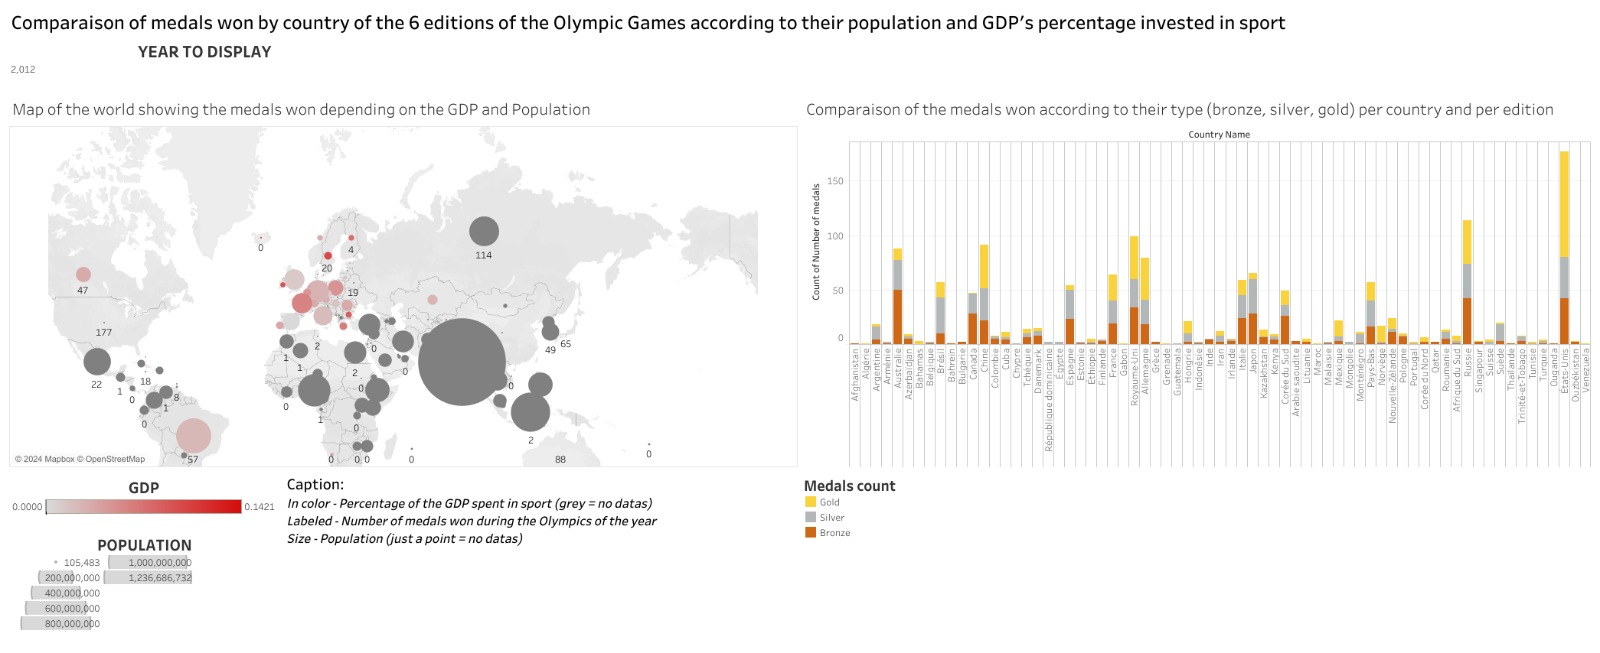
\includegraphics[scale=0.25]{images/datavis-medals-world-tab.jpeg}
		\captionsetup{justification=centering}
		\caption{Aperçu du tableau de bord comprenant les visualisations \textit{Map of the world showing the medals won depending on the GDP and Population} (à gauche) et \textit{Comparison of the medals won according to their type (bronze, silver, gold) per country and per edition} (à droite)}
	\end{figure}
\end{center}

En somme, notre premier ensemble de visualisation prend la forme d'une \enquote{histoire}, permettant une mise en parallèle des différentes représentations :

\begin{center}
	\begin{figure}[H]
		\centering
		\setlength{\belowcaptionskip}{-35pt}
		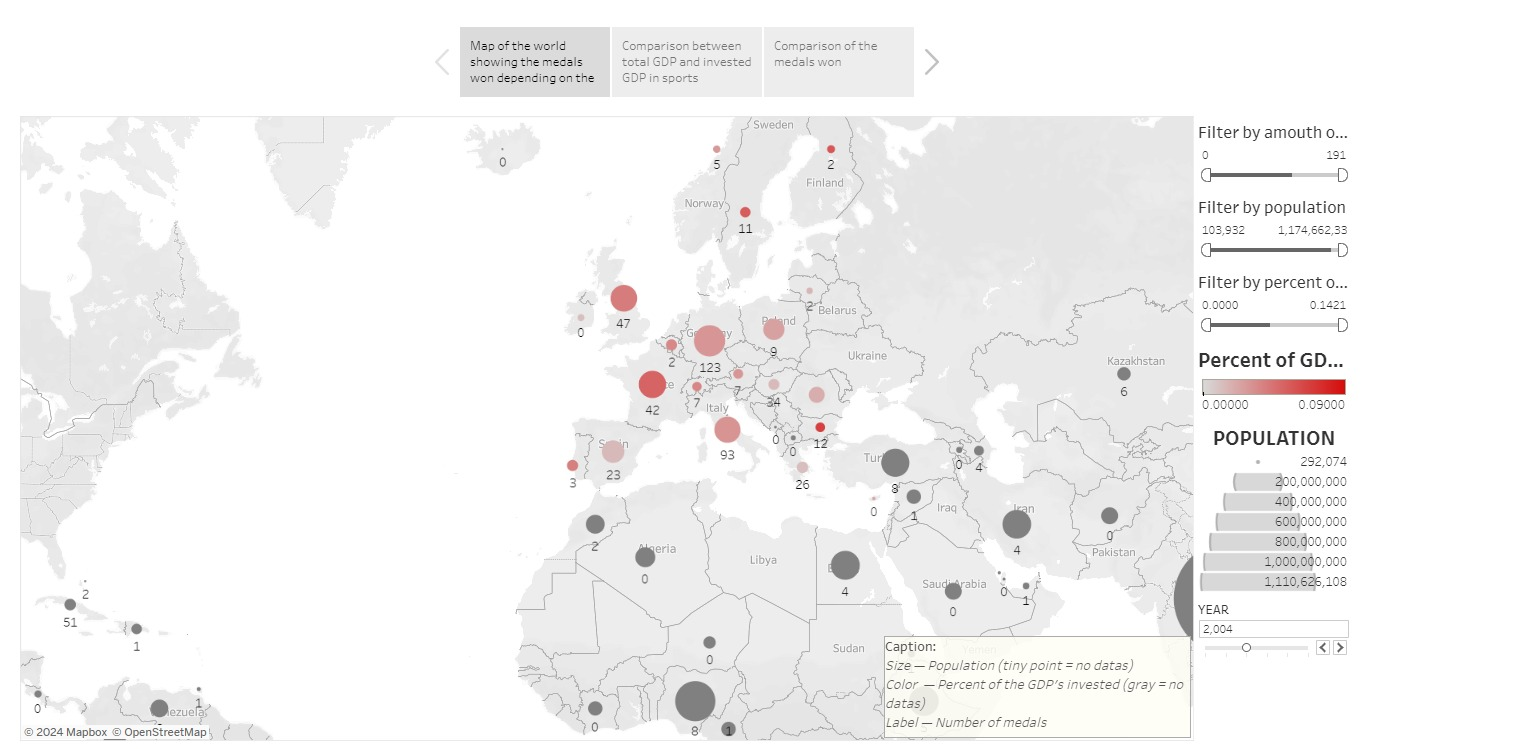
\includegraphics[scale=0.3]{images/datavis-medals-world-map-story.jpeg}
		\captionsetup{justification=centering}
		\caption{Aperçu de la visualisation \textit{Map of the world showing the medals won depending on the GDP and Population} dans le mode \enquote{histoire}}
	\end{figure}
\end{center}

\begin{center}
	\begin{figure}[H]
		\centering
		\setlength{\belowcaptionskip}{-35pt}
		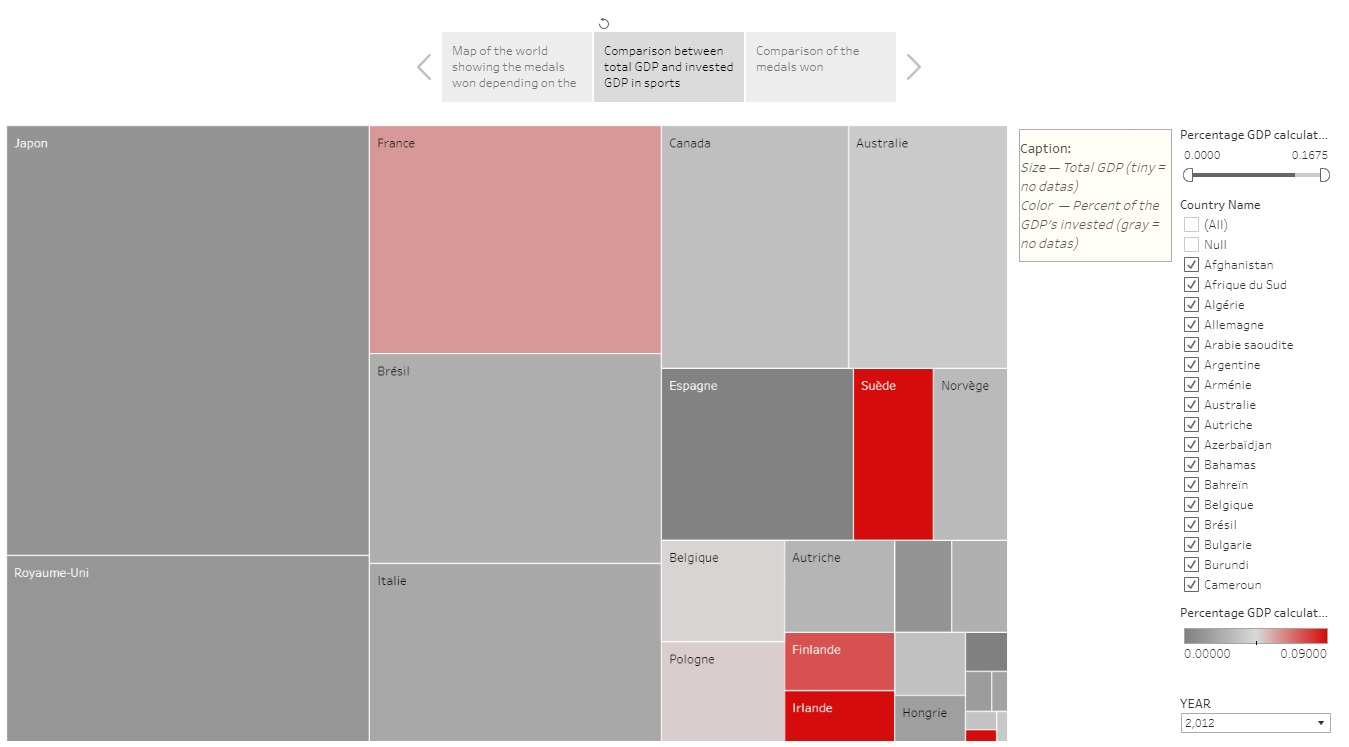
\includegraphics[scale=0.3]{images/datavis-medals-world-treemap-story.jpeg}
		\captionsetup{justification=centering}
		\caption{Aperçu de la visualisation \textit{Comparison between total GDP and invested GDP in sports} dans le mode \enquote{histoire}}
	\end{figure}
\end{center}

\begin{center}
	\begin{figure}[H]
		\centering
		\setlength{\belowcaptionskip}{-35pt}
		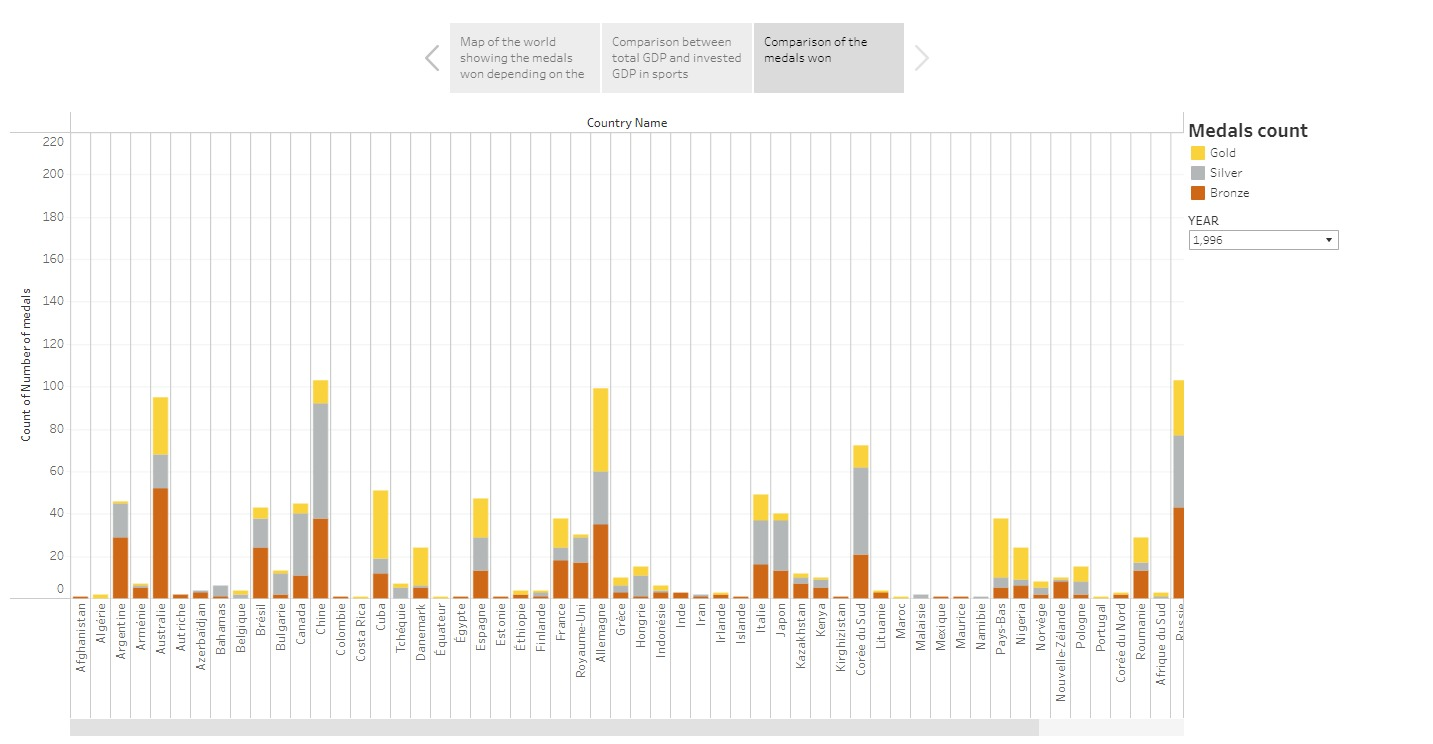
\includegraphics[scale=0.3]{images/datavis-medals-world-histo-story.jpeg}
		\captionsetup{justification=centering}
		\caption{Aperçu de la visualisation \textit{Comparison of the medals won according to their type (bronze, silver, gold) per country and per edition} dans le mode \enquote{histoire}}
	\end{figure}
\end{center}





%





\section{Visualisations du deuxième flux}

\subsection{Répartition des infrastructures de natation}

\subsubsection{Ambition de la visualisation}

Cette visualisation en miroir comprend deux cartes, une de la France métropolitaine, une de l'Angleterre :

\begin{center}
	\begin{figure}[H]
		\centering
		\setlength{\belowcaptionskip}{-35pt}
		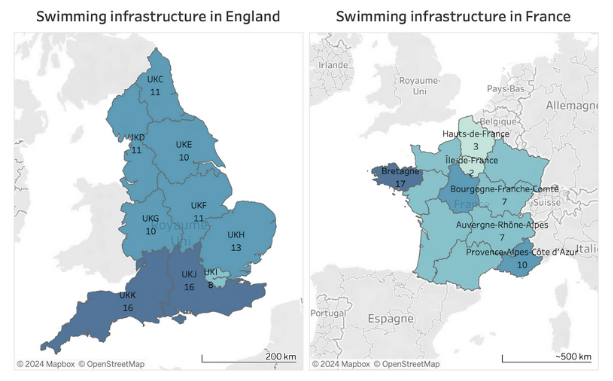
\includegraphics[scale=0.6]{images/datavis-swim-fr-eng.png}
		\captionsetup{justification=centering}
		\caption{Aperçu des visualisations \textit{Swimming infrastructures in England} et \textit{Swimming infrastructures in France}}
	\end{figure}
\end{center}

Elle représente le nombre d'infrastructures de natation par région pour 100.000 habitants. L'investissement se traduit ici par l'accessibilité aux équipements : plus il est d'un niveau élevé, plus la concentration d'équipements (exemplairement des piscines) augmente.

Ce regard présuppose qu'un accès facilité à une infrastructure se traduit par une augmentation du nombre de médailles -- ne prenant donc pas en compte d'autres facteurs potentiellement déterminants (\textit{cf}. \textit{infra} p. \pageref{biais}).

La visualisation est divisée en deux encarts. La première et la deuxième représentent la concentration de piscines sur le territoire français et anglais, rapporté à un coefficient de 100.000 habitants. Les deux cartes partagent une même légende (c'est pourquoi nous prenons la liberté de les présenter simultanément) et partagent une palette de quatre nuances de bleu, permettant une interprétation rapide des ensembles -- en plus des étiquettes affichées.

\subsubsection{Difficultés rencontrées}

Pour un plus grand confort d'interprétation, nous avons choisi de représenter les données aux échelles régionales, non en nous limitant à de simples symboles répartis sur une carte. Pour ce faire, certaines manipulations ont été nécessaires sur les jeux des infrastructures de la France et de l’Angleterre -- directement depuis le logiciel Tableau Public.

Pour la France, la visualisation nécessite la création d'un champ calculé \textit{Pays} ayant pour valeur \enquote{France}, géoréférencé en \enquote{États/régions}. Ce champ a dû ensuite être défini comme \enquote{parent} des données sur les régions. Ces dernières sont alors géoréférencées \enquote{région/province} pour que la visualisation souhaitée puisse être réalisée. Nous pouvons enfin exploiter les données \textit{Swimming pools per 100k inhabitants} en tant que repères de couleur.

La visualisation pour l'Angleterre nécessite une démarche similaire, moyennant une étape supplémentaire. Une fois le champ calculé \textit{Pays} avec pour valeur \enquote{Angleterre} correctement géoréférencé et défini comme \enquote{parent}, les données des régions ne nous permettent pas de créer une visualisation similaire à celle -- pourtant bien fonctionnelle -- de la France.

Il s'agit d'un problème classique de Tableau Public : l'utilisation des coordonnées nous permettait de n'envisager qu'une représentation par points, non pas selon le contour des régions. Nous pensions donc que le nom des régions nous le permettrait mais leur utilisation provoque un conflit avec les régions d'Irlande. La communauté Tableau résout ce type de difficulté en éditant prioritairement les lieux grâce aux options de la carte -- une manipulation vraisemblablement possible seulement sur Desktop Tableau, non pas sur notre version gratuite de Tableau Public.

Une autre solution, plus rudimentaire, présentée par des membres de la communauté Tableau consiste à substituer les noms des entités géographiques, en leur préférant des codes à des noms en langage naturel. Nous avons donc suivi ce procédé en renommant manuellement les régions selon le mode de correspondance suivant :

\begin{center}
	\begin{figure}[H]
		\centering
		\setlength{\belowcaptionskip}{-35pt}
		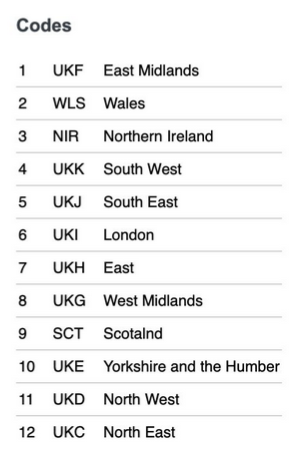
\includegraphics[scale=0.5]{images/datavis-swim-fr-eng-codes.png}
		\captionsetup{justification=centering}
		\caption{Aperçu d'un paramètre de nommage de Tableau Public}
	\end{figure}
\end{center}

Ces conversions faites, nous avons pu géoréférencer la colonne en \enquote{Nuts - Europe} -- seule manière de les faire correctement interpréter par Tableau Public. Nous avons enfin utilisé derechef les données \textit{Swimming pools per 100k inhabitants} comme repères de couleur pour créer une visualisation en miroir avec celle sur les régions de France.

\subsubsection{Regard critique et biais}

\label{biais}Les visualisations accordent une place prépondérante au déterminisme : une simple accumulation d'infrastructures permet-elle de triompher aux compétitions internationales à l'instar des Jeux ? De surcroît, elle rejoue la tension des analyses quantitatives et qualitatives. Qu'en est-il de l'encadrement des athlètes ? De leur temps alloué à la pratique du sport ? Ces équipements sont-ils tous aux normes du Comité International Olympique ?

Sans avoir l'ambition d'être définitive, notre analyse a néanmoins le mérite de poser la question de la simple réduction d'une performance à celle de l'accessibilité -- et de fournir des éléments de réponse.

Le principal biais réside dans les jeux de données à notre disposition. Celui de Kaggle (\textit{cf}. \textit{supra} p. \pageref{kaggle}) porte sur le Royaume-Uni, les infrastructures concernent la seule Angleterre. Ce biais, invalidant \textit{a priori} toute analyse, est néanmoins atténué par notre choix d'identifier des tendances et non des faits arrêtés et binaires -- certainement plus réducteurs dans notre cas.

Notre choix de rapporter les infrastructures à une concentration pour 100.000 habitants limite les biais d'interprétation et de compréhension -- bien que la visualisation ne renseigne pas sur le temps moyen requis pour accéder à l'équipement sportif le plus proche, d'éventuelles disparités au sein même des régions et bien d'autres facteurs encore.

\subsection{Comparaison des médailles remportées en natation}

Notre troisième visualisation exploitant les données du deuxième flux a la forme d'un diagramme en barres :

\begin{center}
	\begin{figure}[H]
		\centering
		\setlength{\belowcaptionskip}{-35pt}
		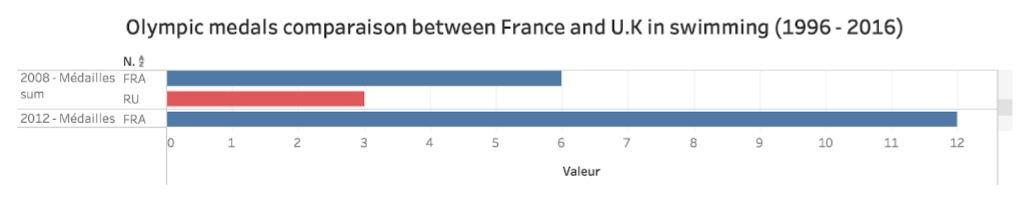
\includegraphics[scale=0.4]{images/datavis-swim-fr-eng-medals.png}
		\captionsetup{justification=centering}
		\caption{Aperçu de la visualisation \textit{Olympic medals comparison between France and England in swimming (1996-2016)}}
	\end{figure}
\end{center}

Sont ici représentées les performances olympiques des deux pays aux épreuves de natation des Jeux entre 1996 et 2016. Pour défiler entre les années, l'utilisateur doit utiliser la molette de sa souris. La visualisation repose sur le nombre total de médailles remportées et exclut donc une spécification de la place occupée sur les podiums. L'Angleterre apparaît en rouge, la France en bleu. Elle regroupe les années, puis les deux pays pour ensuite afficher les médailles. Traduit en application Tableau Public, en colonnes sont les valeurs des mesures et en ligne, les noms des mesures ainsi que les NOC.

Ainsi, pour chaque édition, la réussite sportive peut être efficacement comparée par une simple interprétation visuelle. Par voie de conséquence, cette visualisation rend possible la confrontation avec notre hypothèse de l'existence d'un lien entre les investissements et les résultats aux Jeux.

\subsubsection{Difficultés rencontrées}

D’un point de vue technique, la réalisation de cette visualisation n’a pas souffert de difficultés.

\subsubsection{Regard critique et biais}

Le mode de représentation de cette visualisation fait l'objet d'une insatisfaction, contraint par la taille de la fenêtre : il faut faire défiler les années pour prendre connaissance de l'ensemble des résultats, limitant ainsi une interprétation globale au premier abord.

Cette datavisualisation offre des éclairages pertinents. Il est évident qu'une disjonction se produit entre notre hypothèse initiale, mise en valeur par les autres visualisations, et celle spécifiquement axée sur les infrastructures de piscine en France et en Angleterre.

Aucune interprétation linéaire des résultats obtenus n'est apparente. Ces derniers réaffirment, au-delà d'un seuil de performance minimale et optimale depuis 2008, la part irréductible de l'impondérable dans la performance sportive, faite de hasards, de déconvenues et d'exploits.

Voici en somme notre deuxième ensemble de visualisation, prenant la forme d'un tableau de bord :

\begin{center}
	\begin{figure}[H]
		\centering
		\setlength{\belowcaptionskip}{-35pt}
		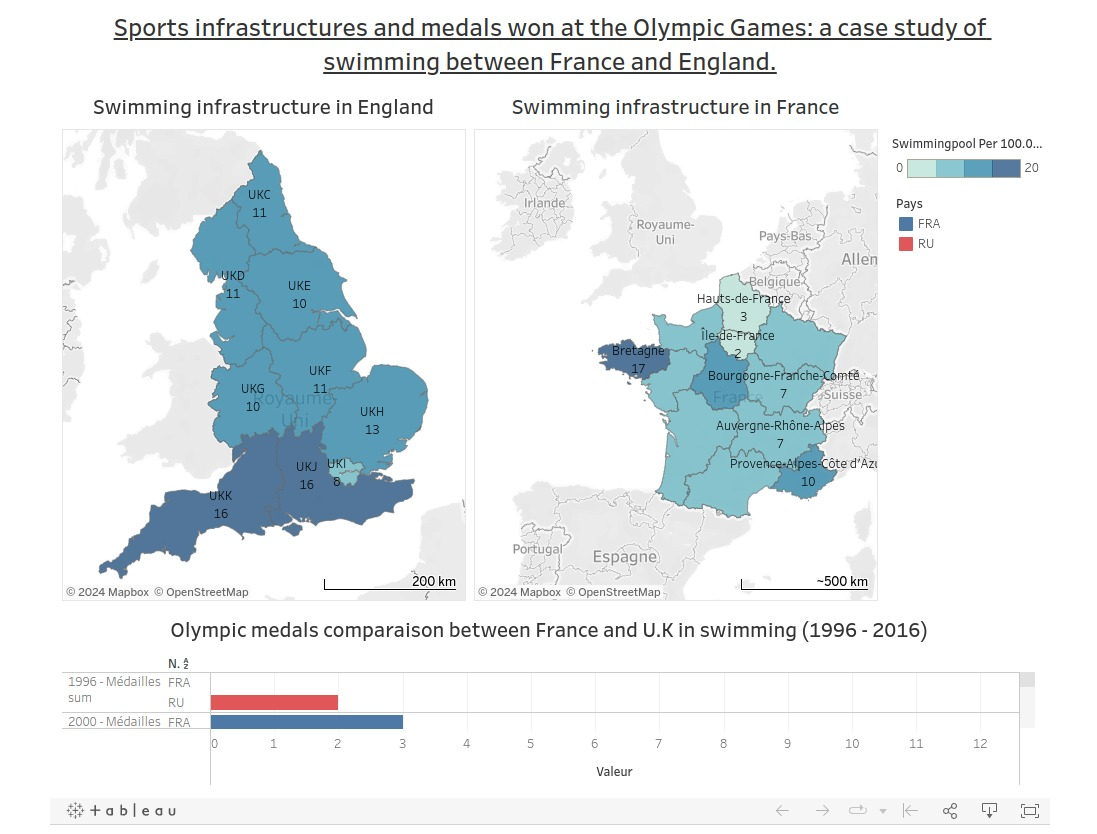
\includegraphics[scale=0.35]{images/datavis-swim-tab.jpeg}
		\captionsetup{justification=centering}
		\caption{Aperçu du tableau de bord \textit{Sports infrastructures and medals won at the Olympic Games: a case study of swimming between France and England}}
	\end{figure}
\end{center}





%





\section{Une synthèse analytique}

Les visualisations que nous avons réalisées nous permettent de matérialiser plusieurs jeux de données représentant les relations entre investissements et résultats aux Jeux Olympiques. Mais nous permettent-elles d’esquisser une vérité satisfaisante ?

\subsection{Visualisations du premier flux}

\label{nuance}Si nous faisons une rapide synthèse de ce premier ensemble de visualisations, Nous observons la logique suivante sur le plan macroscopique : plus un pays investit dans le sport, plus il remporte de médailles aux Jeux Olympiques. Cette assertion contient néanmoins quelques nuances sur un aspect plutôt microscopique -- notamment au niveau des pays les données en lien avec l’investissement manquent.

\subsubsection{Le cas de la Chine}

Attardons-nous un instant sur un fait important : la Chine, faisant partie des BRICS, possède un nombre de médailles extrêmement élevé par rapport aux pays développés. Elle est de fait la principale concurrente des États-Unis à partir des années 2000. Cela peut être dû à l'importante population de la Chine, mise en exergue par la visualisation du monde (\textit{cf}. \textit{supra} p. \pageref{map}).

Cependant, un contre-exemple de taille vient infirmer cette hypothèse. L'Inde a beau posséder la deuxième plus grande population mondiale, elle n'est pas aussi performante aux Jeux. La Chine constitue donc la première nuance visible de notre hypothèse de départ : il reste difficile d’expliquer son succès si l’on se fonde sur nos seules données économiques et démographiques.

\subsubsection{Le cas des anciens pays de l’URSS, de la Yougoslavie et du Kenya}

Une grande partie de pays concourant aux Jeux depuis 1996 possède des résultats étonnamment élevés si nous les comparons à ceux des pays développés. Sont concernés les pays de l'ex-Yougoslavie et de l'URSS -- citons en guise d'exemple la Russie, la Hongrie, l'Ukraine ou l'Azerbaïdjan -- et plus au sud, le Kenya. Depuis les années 2000, ces pays s'approchent, voire dépassent, la dizaine de médailles remportée par édition. 

Si nous cherchons des éléments démographiques explicatifs, la Russie possède une population de 150 millions d'habitants -- or le Kenya et l'Ukraine n'en comptent pas plus d'une soixantaine, tandis que la Hongrie et l'Azerbaïdjan n'en comptent pas plus d'une dizaine. Par ailleurs, le seul cas de l'Inde nous a montré qu'un indice de population élevé ne saurait être seul un argument démonstratif convaincant.

Ce peut être dû aux spécificités de la culture sportive des pays : le Kenya remporte l'essentiel de ses médailles en athlétisme et l'Azerbaïdjan en haltérophilie. Enfin, l'URSS était un adversaire majeur des États-Unis lors des Jeux avant l'entrée en concurrence sérieuse de la Chine. Nous pouvons supposer que les pays membres de l'URSS ont conservé les vestiges de cette culture de la performance.
\newline

En somme, si les pays qui investissent le plus dans le sport -- exemplairement les pays développés -- ont de plus grandes chances de réussite aux Jeux. Nonobstant, des exceptions à l'instar de la Chine ou des pays d'Europe de l'Est forcent à nuancer cette assertion.





%





\subsection{Visualisations du second flux}

Ce deuxième ensemble de visualisations ambitionnait d'éprouver notre hypothèse à propos d'épreuves sportives précises et sur des territoires plus réduits -- en l'occurrence la France métropolitaine et l'Angleterre.

Si l'assertion selon laquelle plus un pays investit dans le sport, plus il remporte de médailles peut trouver des éléments de confirmation à l'échelle macroscopique -- en prenant en compte les nuances mentionnées \textit{supra} (\textit{cf}. p \pageref{nuance}), sa pertinence est moins évidente au regard de notre étude comparative.

Les visualisations nous permettent de constater que l'accessibilité aux équipements sportifs relatifs à la natation est plus saillante en Angleterre qu'en France métropolitaine. Néanmoins, le nombre de médailles remportées par les deux pays est très proche sur le temps long (soit l'ensemble des éditions retenues sur lesquelles portent notre travail).

Le fait de plus précisément s'intéresser à une discipline sportive et aux investissements liés tend donc à infirmer notre hypothèse -- bien entendu selon les données à notre disposition.





%





\chapter{Remarques et péripéties}

\section{Typage de données}

Un grand défi du traitement a été le typage de données, autant pour Dataiku que pour Tableau Public. Nous découvrions ces deux logiciels et parvenir à les faire dialoguer n'a pas été sans peine (exemplairement à propos des coordonnées, \textit{cf}. \textit{supra} p. \pageref{casse}). Dataiku retypait des données automatiquement en dépit de nos modifications manuelles et chaque exécution de recette et réalisation de datavisualisation était mue par le risque d'un bogue de typage et l'obligation d'intervenir de nouveau dans les flux.

\section{Bogue Dataiku}

La semaine du 22 janvier a été le lieu d'une mauvaise surprise. Alors que nous voulions examiner le premier flux sur Dataiku pour rédiger le présent journal de bord, il nous a été subitement impossible de visualiser les jeux. L'interface générale fonctionnait, nous pouvions voir le flux, cliquer sur les icônes de recettes ou de jeux mais ce faisant, la partie de l'écran devant afficher les données était vide. L'erreur renvoyée est la suivante :

\begin{center}
	\begin{figure}[H]
		\centering
		\setlength{\belowcaptionskip}{-35pt}
		
\includegraphics[scale=0.49]{images/bogue.png}
		\caption{Bogue rencontré sur le logiciel Dataiku}
	\end{figure}
\end{center}

Il est probable que cette erreur ait été créée après l'installation d'une version de \textit{Java Development Kit} (à l'occasion d'un cours de XQuery) supérieure à celle prise en charge par Dataiku, sur la machine où a été réalisé l'ensemble du traitement des données. Il aurait fallu rétrograder la version de JDK mais nous craignions que celle manipulation n'entraîne des difficultés sur l'ensemble des projets dépendants de JDK.

Nous avons été forcés de nous appuyer sur d'autres ordinateurs pour consulter les flux et terminer le traitement (la réalisation du deuxième flux n'avait alors pas commencé, et celle du premier n'était pas tout à fait achevée). Cela a causé d'importants soucis organisationnels en cette fin de mois.

\section{Sur l'utilité de Wikidata}

Au cours du traitement Wikidata s'est révélé être un outil formidable pour l'enrichissement et le traitement des données. Le système de construction des requêtes SPARQL nécessite une certaine prise en main mais nous permet de très larges interrogations de la base de données.

Les jeux générés sont très bien formés et présentent un intérêt certain pour correctement réaliser des jointures à l'aide des nombreux codes, labels et identifiants récupérables.





%





\chapter{Un mot de conclusion}

Ce projet a été le lieu de nombreuses complications et péripéties mais nous ne saurions faire l'impasse sur les opportunités et perspectives de travail dont il témoigne. Nous avons la certitude qu'avec un -- même maigre -- renfort d'effectifs, de ressources financières et de temps, nous aurions pu trouver des jeux de données mieux formés, plus complets et ainsi produire des visualisations plus parlantes et pertinentes.

Nous avons conscience des nombreux biais et manquements qui émaillent nos productions finales (manque de données, chaînes de caractères à la fois en français et en anglais, glissement des régions de France et du Royaume-Uni vers les régions de France métropolitaine et d'Angleterre) mais nous pensons avoir démontré qu'un travail de qualité à propos des Jeux Olympiques est possible et éclairant sur les donnes économiques et sportives des pays.





%





\chapter{Sitographie}
\printbibliography[heading=none]
\newpage

%(\textit{cf}. \textit{supra} p. \pageref{nongrata})

\end{document}